%!TEX root = ../thesis.tex
%*******************************************************************************
%*********************************** Analysis Overview *********
%*******************************************************************************

\chapter{Reinterpretation in the pMSSM}\label{ch:pmssm}

\ifpdf
    \graphicspath{{chapter-pmssm/Figs/Raster/}{chapter-pmssm/Figs/PDF/}{chapter-pmssm/Figs/}}
\else
    \graphicspath{{chapter-pmssm/Figs/Vector/}{chapter-pmssm/Figs/}}
\fi

After having discussed to some extent efforts and methods to reinterpret ATLAS searches for \gls{susy}, this chapter presents a reinterpretation of the 1-lepton analysis in the \gls{pmssm}. The truth analysis and simplified likelihoods discussed in~\cref{ch:preservation,ch:simplify}, respectively, are instrumental for the following sections. 

\section{Motivation}

In today's searches for \gls{bsm} physics, it is common to use simplified models as a way of avoiding to necessity to deal with high-dimensional parameter spaces that are extremely challenging to sample and compare to data in an exhaustive way. The simplified model approach has also been used in the second part of this work, where results of the interpretation of the 1-lepton analysis in the $\charg\neutr\rightarrow Wh\lsp\lsp$ model have been presented. As has been discussed in~\cref{sec:simplified_models}, simplified models are however by no means complete \gls{susy} models and only serve as proxies for more complex and realistic \gls{susy} scenarios. As such, simplified model limits cannot trivially be translated into limits on model parameters of a more complete \gls{susy} model. Large-scale reinterpretations are necessary to understand the constraints today's \gls{susy} searches set on realistic \gls{susy} scenarios. 

One class of more complete models, focussing on phenomenologically viable models, is the \gls{pmssm}, introduced in~\cref{sec:theory_pmssm}. With its 19 parameters it offers much more complex \gls{susy} scenarios while still being of somewhat manageable dimensionality. Still, large-scale reinterpretations in the \gls{pmssm} are computationally challenging and require a set of approximation as those introduced in~\cref{ch:preservation,ch:simplify}.

Large-scale reinterpretations in the \gls{pmssm} using a collection of relevant ATLAS \gls{susy} searches not only allow to assess the sensitivity of the ATLAS \gls{susy} search program towards more realistic \gls{susy} scenarios, but can also potentially reveal interesting regions of the parameter space not yet covered by the current search programme. Moreover, such reinterpretations allow to demonstrate the sensitivity of simplified model searches beyond the simplified models they are originally interpreted in, thereby justifying the use of simplified models as proxies for more complete \gls{susy} scenarios. In addition, reinterpretations in the \gls{pmssm} can be used to connect the ATLAS \gls{susy} searches with dark matter constraints from non-collider experiments, as well as Higgs and flavour measurements. \unsure{might want to tweak this last sentence} 

Although the following sections will be restricted to a reinterpretation of the 1-lepton search presented in the second part of this thesis, efforts are ongoing in ATLAS to perform large-scale reinterpretations using a majority of the full Run~2 ATLAS \gls{susy} searches. These efforts will most likely result in one of the most comprehensive set of ATLAS constraints on \gls{susy} yetope.

\section{Truth analysis}\label{sec:truth_analysis}

As discussed in~\cref{ch:preservation}, the reinterpretation of an analysis involves re-executing the analysis pipeline in order to derived signal rate estimates in all regions. In large-scale reinterpretations, running a \textsc{Recast} implementation on all signal models considered is not computationally feasible and instead a \textit{truth-level} analysis is performed for most signal models sampled. The truth-level analysis skips the detector simulation and uses generator-level objects instead. Any detector-level effects and inefficiencies will thus not be reflected in truth-level observables. In order to reproduce the kinematic distributions observed in the full analysis (using reconstruction-level objects), a dedicated \textit{truth smearing}---discussed in detail in~\cref{sec:truth_smearing}---is applied.

\subsection{Truth selection}\label{sec:truth_selection}

All signal and control regions considered in the original 1-lepton search are implemented at truth-level using \textsc{SimpleAnalysis}. The exact implementation is publicly available at \reference\cite{HEPdata_1Lbb} and was already used in~\cref{ch:uncertainties} for the derivation of a number of the theory uncertainties in the full analysis.

Although a number of object definitions introduced in~\cref{sec:object_definitions} are not well-defined at truth-level, they are nonetheless specified in the truth-level implementation as the subsequent truth smearing may depend on them. Additionally, as discussed in~\cref{sec:reinterpretations}, the full specification of the original analysis event selection allows for simpler reinterpretations by efforts outside of the ATLAS collaboration that generally do not have access to the full original analysis software.

All observables used in the analysis are computed using truth-level quantities. An overlap removal procedure following the same prescription as described for the reconstruction-level analysis is performed, \ie especially also using the same shrinking cone definitions introduced in~\cref{sec:overlap_removal}. Overlap removal step removing electrons sharing a track with a muon is approximated by using a distance parameter of $\Delta R = 0.01$ between the objects. 

\subsection{Truth smearing}\label{sec:truth_smearing}

The general assumption of the truth smearing applied in the following is that the detector response roughly factorises into the responses of single particles. This allows to use detector performance results provided by the \textit{combined performance groups} in ATLAS in order to construct detector response maps parameterised in different observables for each physics object. Detector response maps include object reconstruction and identification efficiencies as well as scale factors to correct for differences between \gls{mc} and observed data. Likewise, effects from the finite resolution of energy measurements in the detector are modelled through energy resolution maps. In the following, the 4-vector components of electrons, muons, jets and $\etmiss$ are smeared.

In the case of truth electrons, the identifications efficiencies considered are parameterised in $\eta$ and $\pt$ as well as the identification working point used. In $\eta$, nine fixed-width bins are used. In $\pt$, six bins are implemented and a linear interpolation between two adjacent $\pt$-bins is used to get the efficiency for the given $\pt$ of each truth electron. The probability of finding a fake electron in a truth jet is estimated through a similar two-dimensional map depending on the truth jet $\eta$ and $\pt$, again using fixed-width bins in $\eta$ and linear interpolation in $\pt$. The range of the $\pt$ interpolation for identification efficiencies and fake rates extends from $\SI{7}{\GeV}$ to $\SI{120}{\GeV}$. If the truth $\pt$ of the electron is outside of that range, the identification efficiency and fake rate from the respective bound of the corresponding $\eta$-bin are used. The probability for misidentifying an electron as a photon is estimated using different fixed values for the barrel and end-cap regions. Finally, the transverse energy of the electron is smeared using a random number drawn from a Gaussian distribution with mean corresponding to the truth value and a standard deviation corresponding to the $\eta$- and $\pt$-dependent energy resolution.  

For truth muons, the identification efficiencies are also parameterised in $\eta$ and $\pt$ as well as the identification working point used. Similar to truth electrons, the  $\pt$ of the muon is smeared using a random number drawn from a Gaussian distribution with mean corresponding to the true transverse momentum, and standard deviation corresponding to the momentum resolution. The momentum resolution of combined truth muons is computed from the measured resolutions in the \gls{id} ($\sigma_\mathrm{ID}$) and \gls{ms} ($\sigma_\mathrm{MS}$) as
\begin{equation}
	\sigma_\mathrm{CB} = \frac{\sigma_\mathrm{ID}\sigma_\mathrm{MS}}{\sqrt{\sigma_\mathrm{ID}^2 + \sigma_\mathrm{MS}^2}},
\end{equation}
where $\sigma_\mathrm{ID}$ and $\sigma_\mathrm{MS}$ are parameterised in $\eta$ and $\pt$.

The transverse momentum of truth jets is smeared using a Gaussian with standard deviation equal to the \gls{jer}, provided in a map parameterised in five bins in $\eta$ ranging from $\vert\eta\vert = 0$ to $\vert\eta\vert = 4.5$. Following~\cite{Aad:2020flx}, jet energy resolutions are provided using parameterisations of a noise $N$, stochastic $S$ and constant $C$ term for each of the seven bins in $\vert\eta\vert$, such that the resolution can be computed as
\begin{equation}
	\frac{\sigma(\pt)}{\pt} = \frac{N}{\pt}\oplus\frac{S}{\sqrt{\pt}}\oplus C.
\end{equation}
Only truth jets with $\SI{10}{\GeV} < \pt < \SI{1.5}{\TeV}$ are smeared. For truth jets with $\pt > \SI{20}{\GeV}$, the flavour tagging efficiency is considered using efficiencies parameterised in $\eta$, $\pt$ and the \textsc{MV2c10} working point (introduced in~\cref{sec:object_definitions}) used, measured in fully reconstructed simulated $\ttbar$ events~\cite{FTAG-2018-01}.

Finally, the smeared missing transverse energy is computed using the the transverse momenta of all smeared truth objects in the event, including an approximation for the track soft term. The latter is approximated using results from $Z\rightarrow e^+e^-$ events, allowing to infer a distribution of the mean soft term projected in the direction longitudinal to the total transverse momentum of all hard objects in an event, $\boldsymbol{p}_\mathrm{T}^\mathrm{hard}$. The measured resolution parallel and perpendicular to $\boldsymbol{p}_\mathrm{T}^\mathrm{hard}$ is then used to smear the nominal soft track value.
 
 
 \section{Validation of truth analysis}
 
 \subsection{Validation at loose preselection}

  \begin{figure}
	\centering
	\begin{subfigure}[b]{0.45\linewidth}
		\centering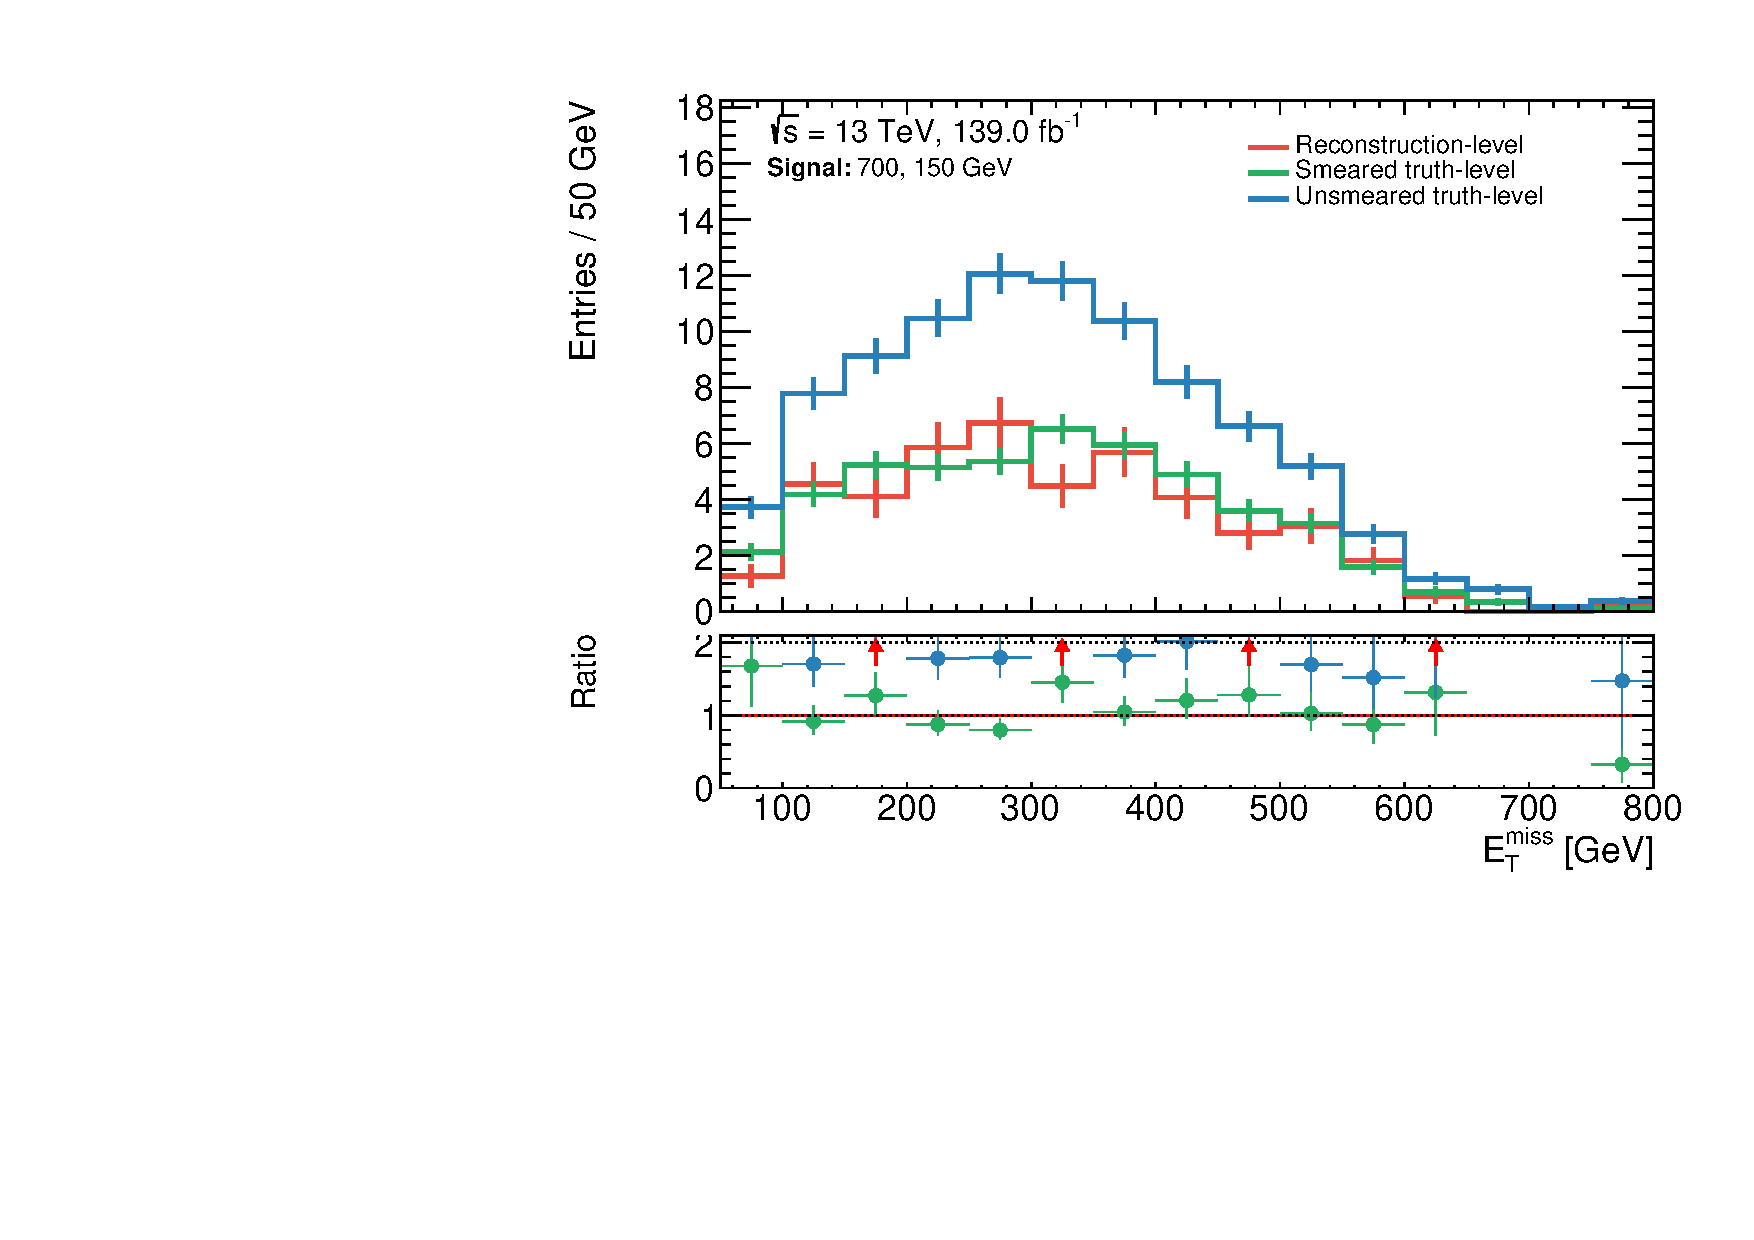
\includegraphics[width=\textwidth]{met_C1N2_Wh_hbb_700p0_150p0_smeared.pdf}
	\end{subfigure}\hfill
	\begin{subfigure}[b]{0.45\linewidth}
		\centering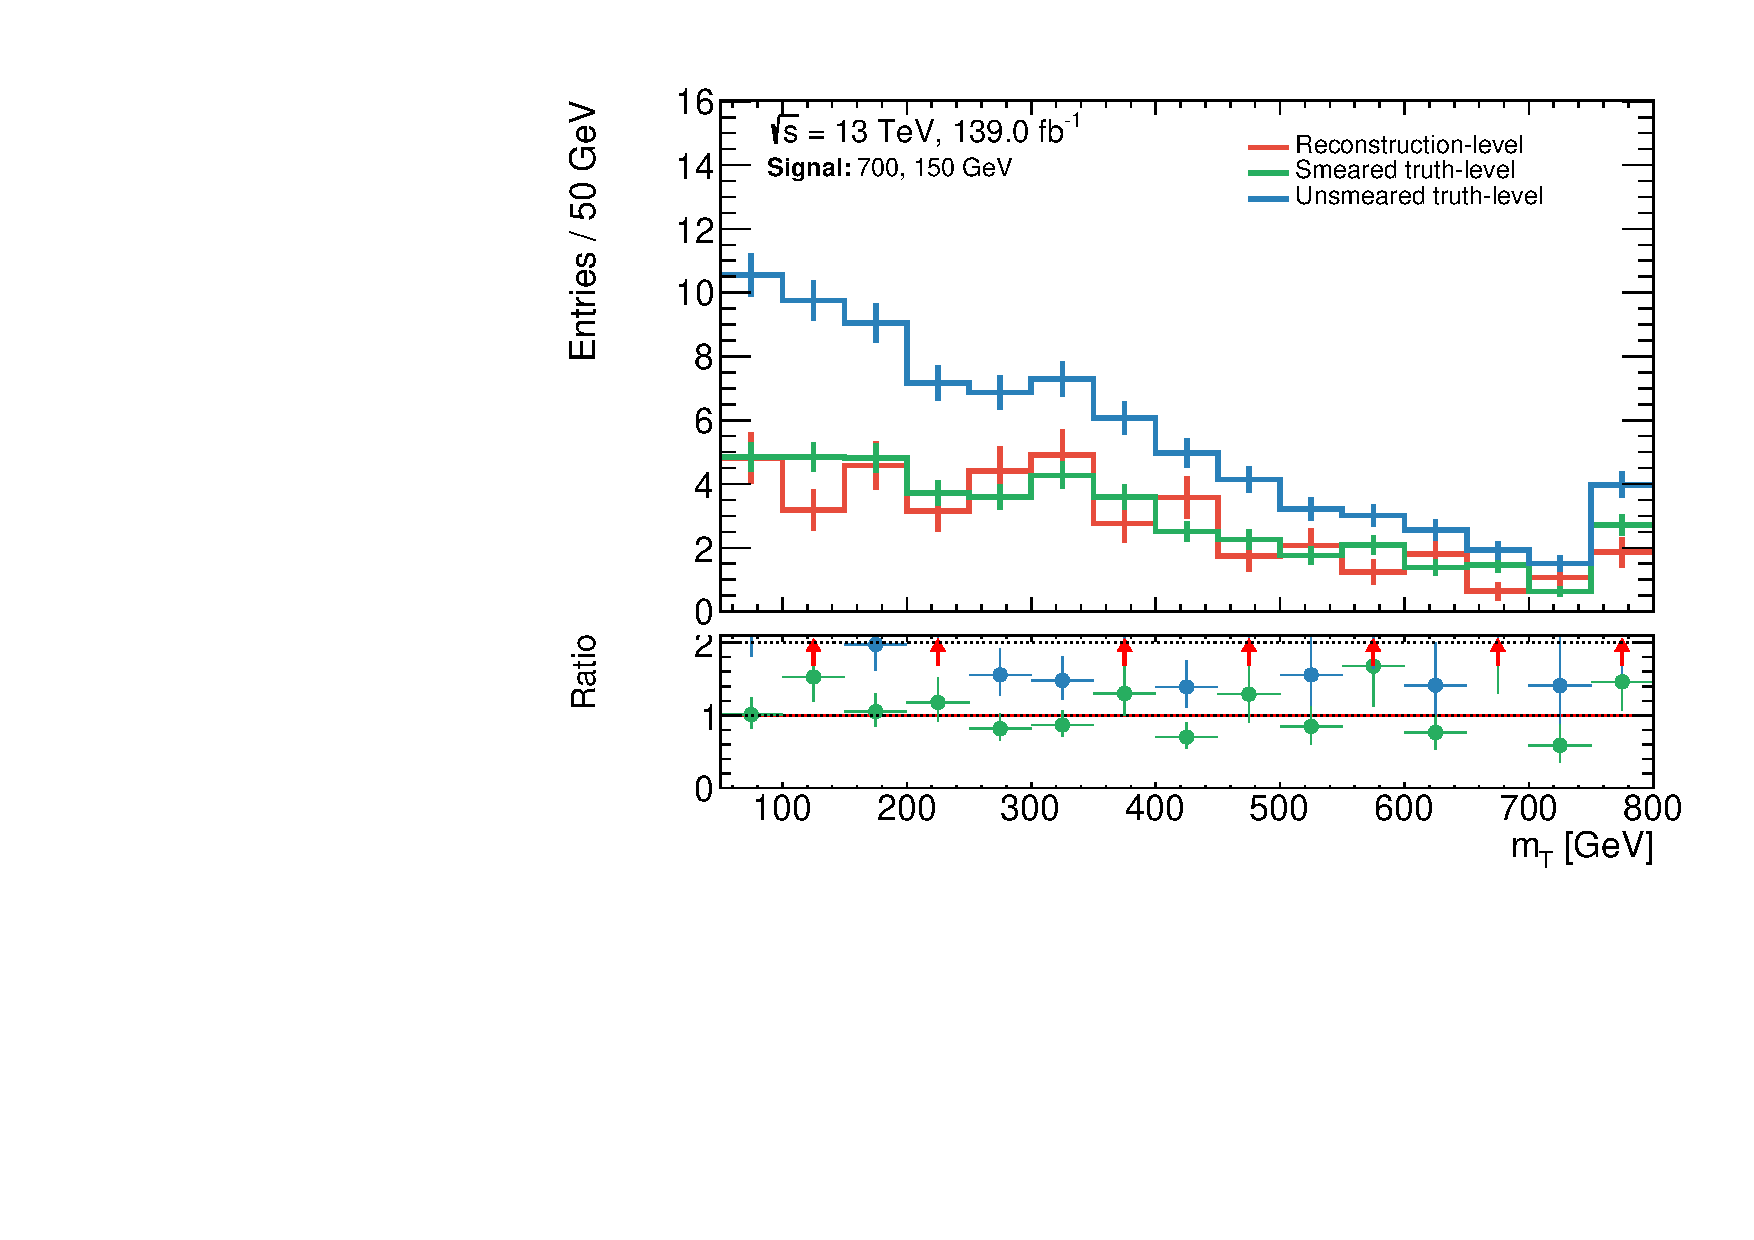
\includegraphics[width=\textwidth]{mt_C1N2_Wh_hbb_700p0_150p0_smeared.pdf}
	\end{subfigure}\hfill
	\begin{subfigure}[b]{0.45\linewidth}
		\centering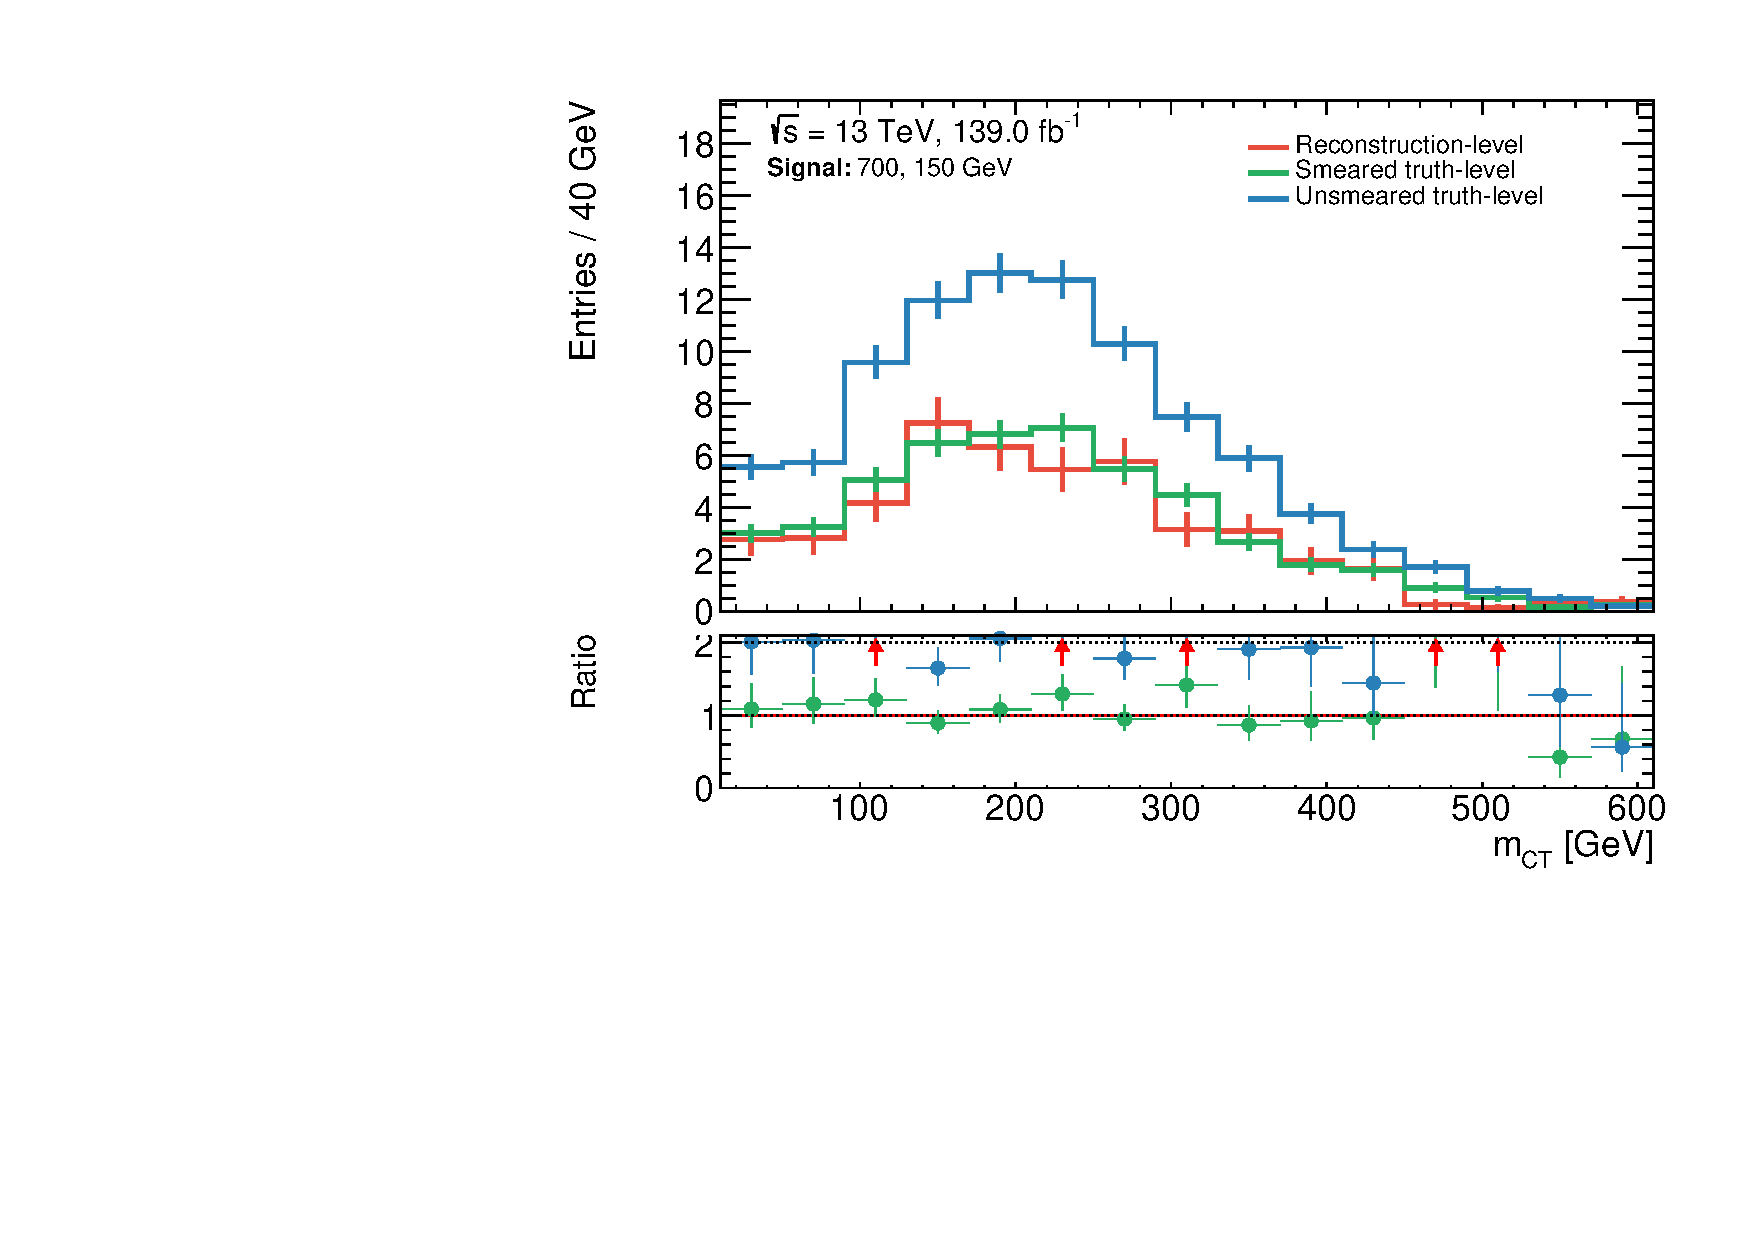
\includegraphics[width=\textwidth]{mct_C1N2_Wh_hbb_700p0_150p0_smeared.pdf}
	\end{subfigure}\hfill
	\begin{subfigure}[b]{0.45\linewidth}
		\centering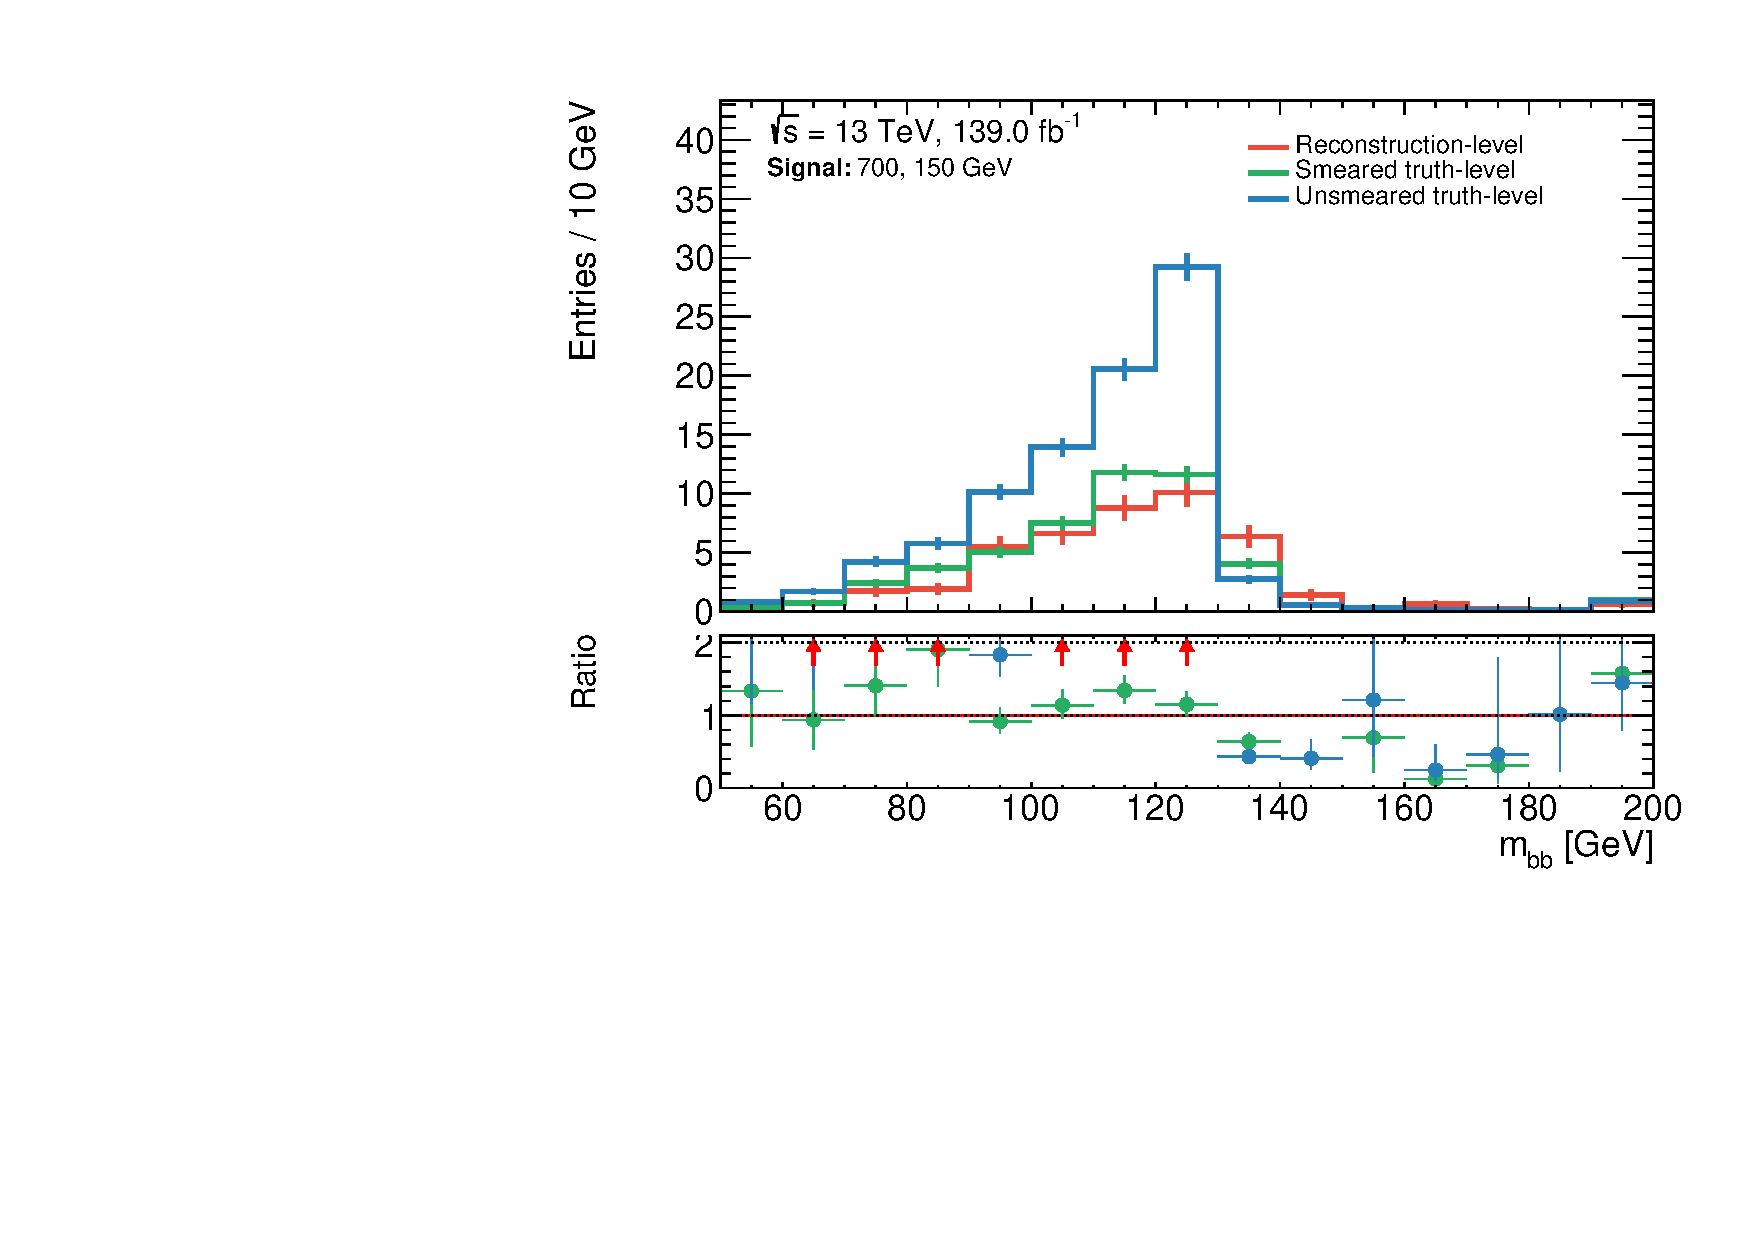
\includegraphics[width=\textwidth]{mbb_C1N2_Wh_hbb_700p0_150p0_smeared.pdf}
	\end{subfigure}\hfill
	\begin{subfigure}[b]{0.45\linewidth}
		\centering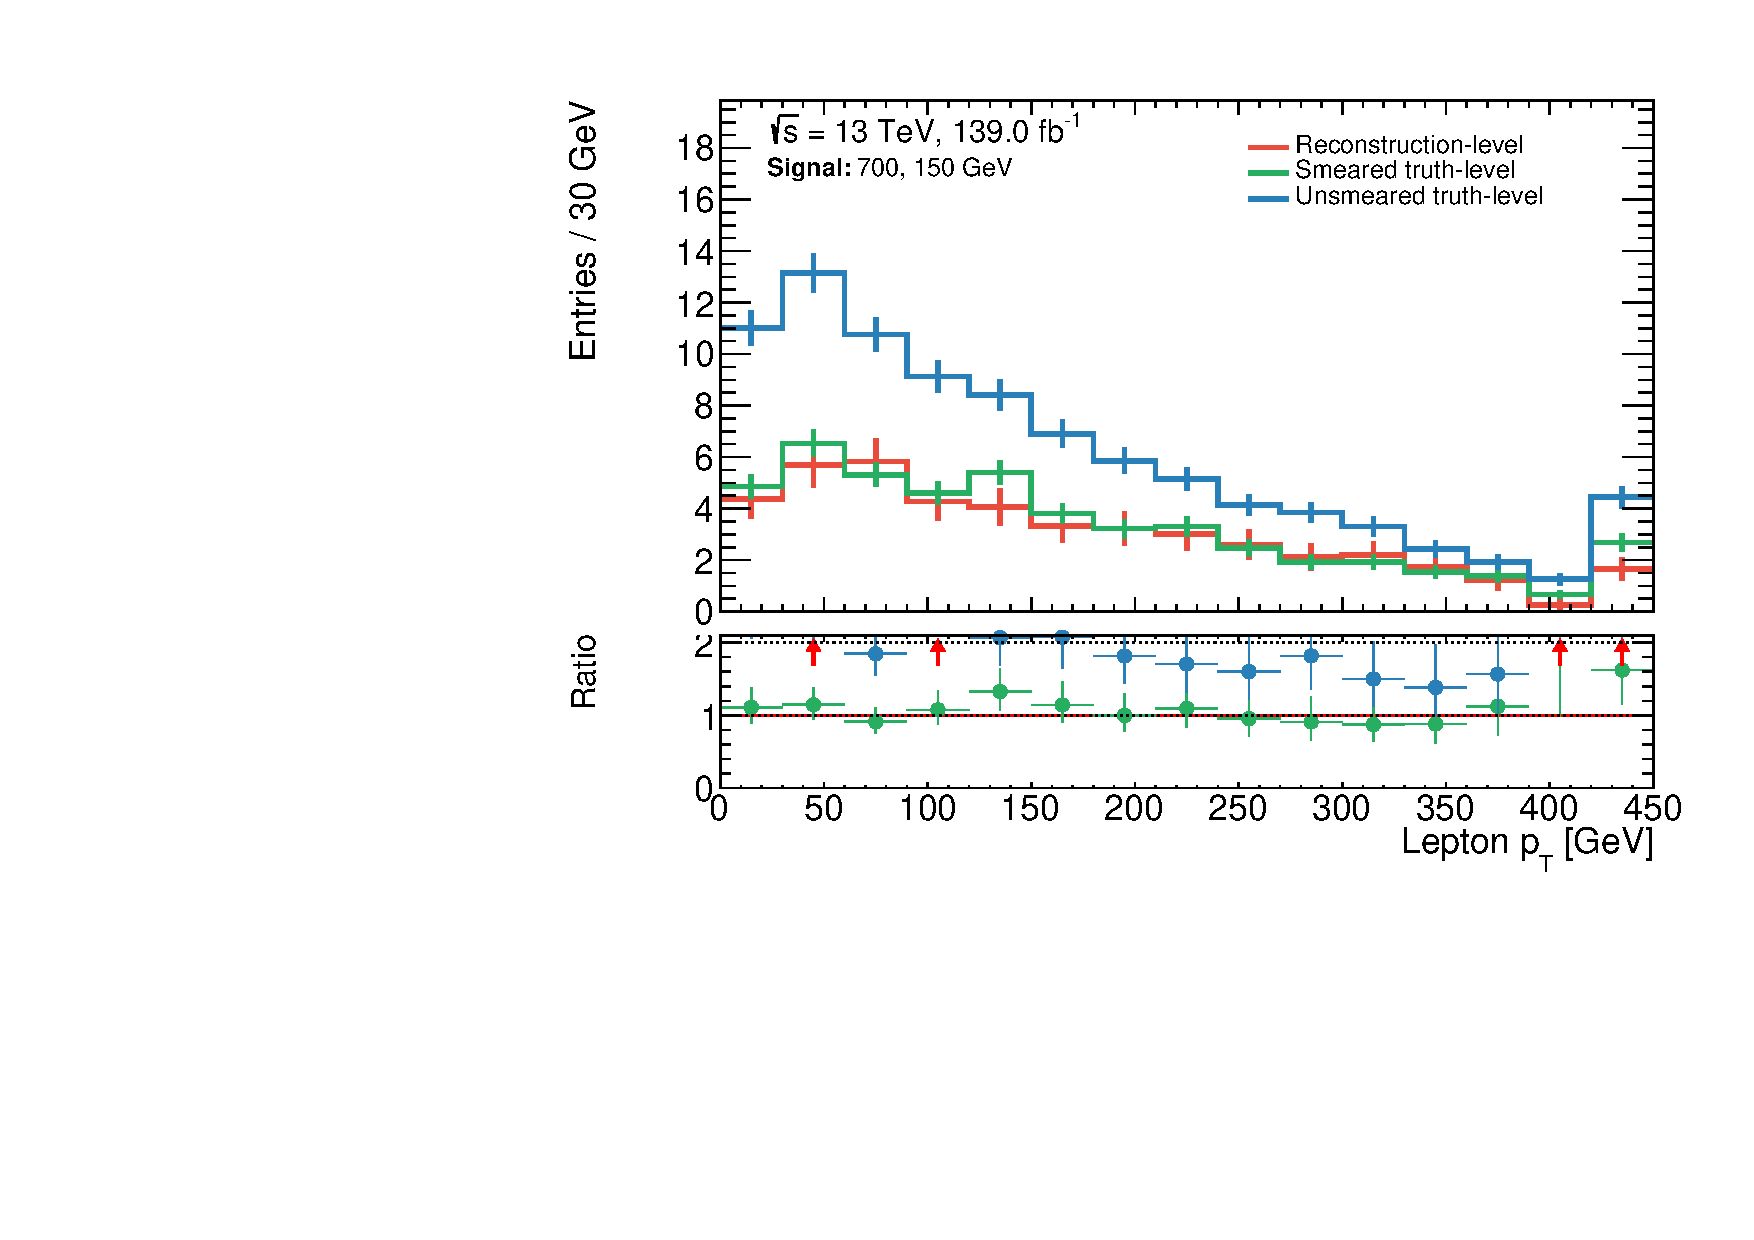
\includegraphics[width=\textwidth]{lep1Pt_C1N2_Wh_hbb_700p0_150p0_smeared.pdf}
	\end{subfigure}\hfill
	\begin{subfigure}[b]{0.45\linewidth}
		\centering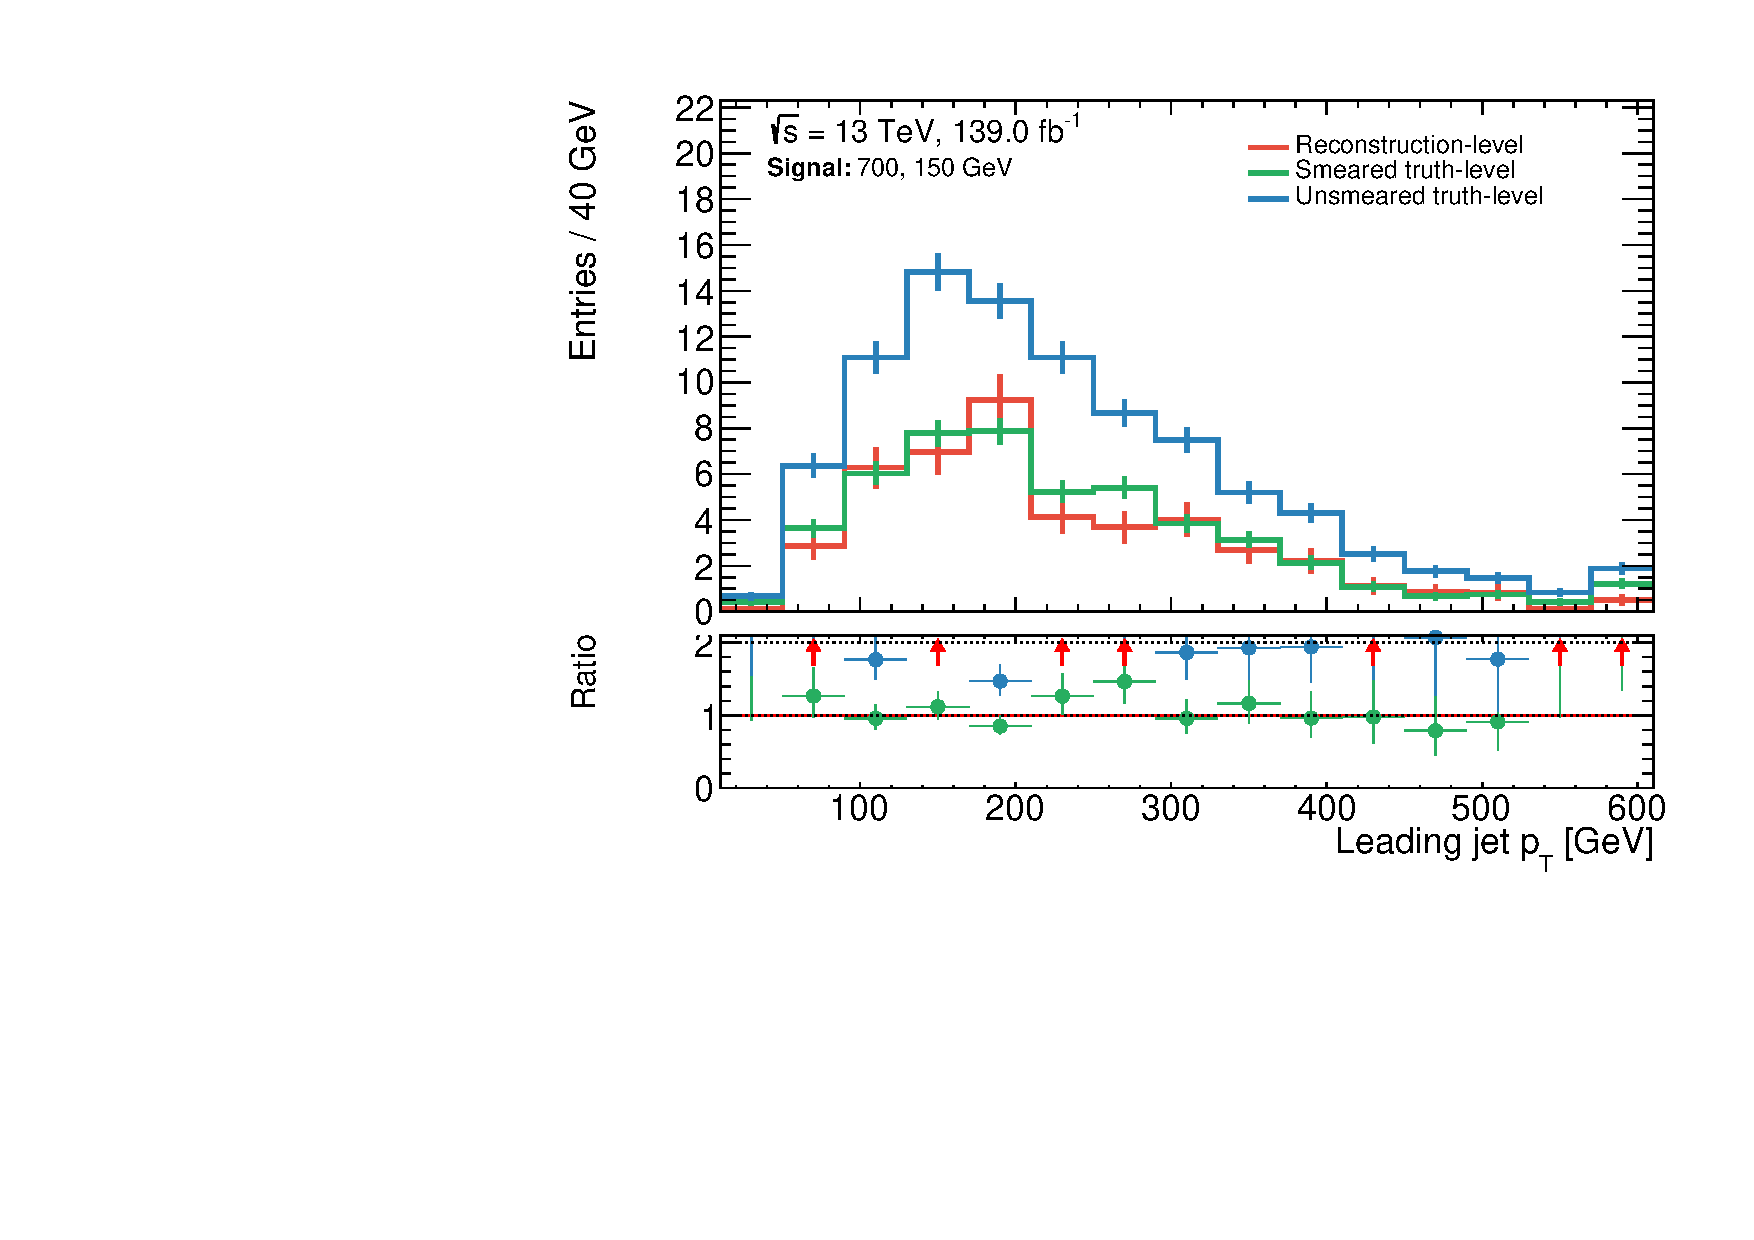
\includegraphics[width=\textwidth]{jet1Pt_C1N2_Wh_hbb_700p0_150p0_smeared.pdf}
	\end{subfigure}\hfill
	\begin{subfigure}[b]{0.45\linewidth}
		\centering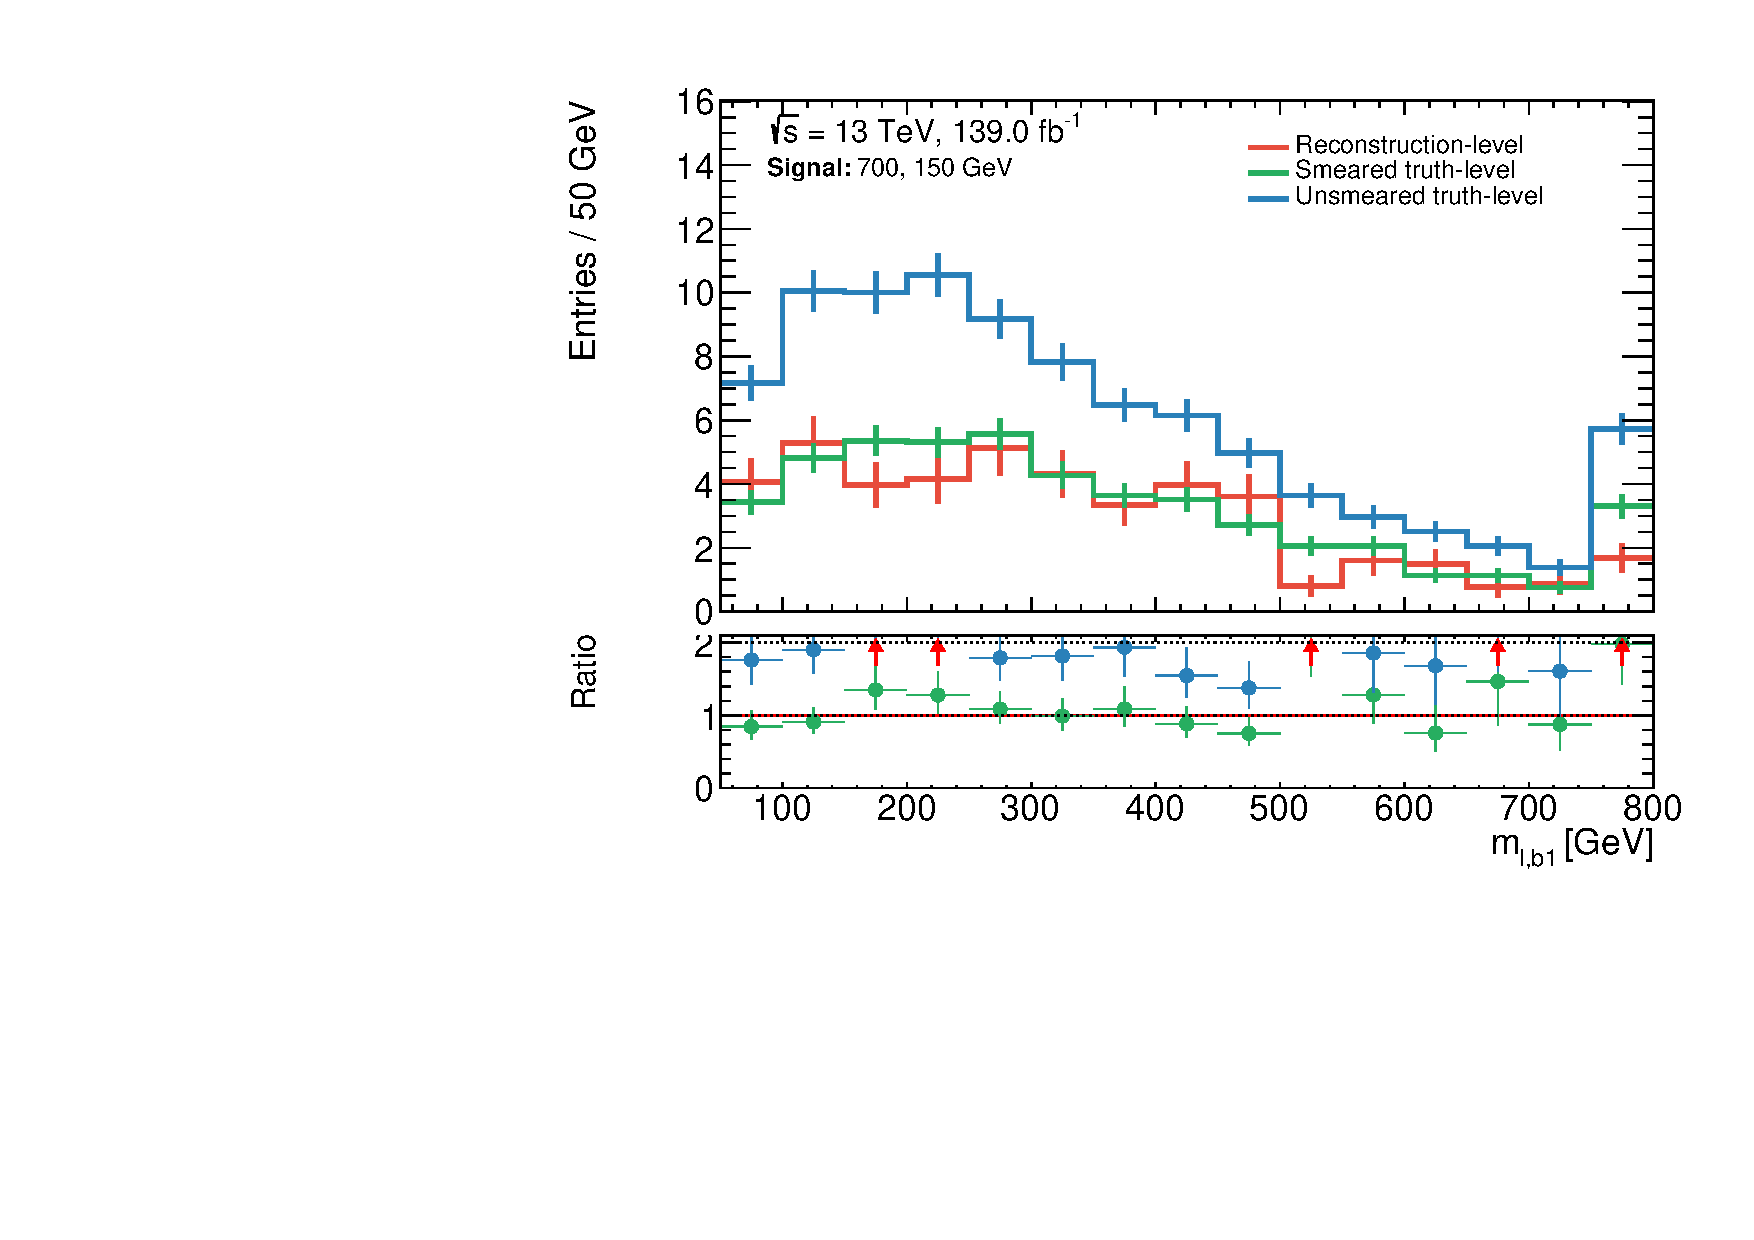
\includegraphics[width=\textwidth]{mlb1_C1N2_Wh_hbb_700p0_150p0_smeared.pdf}
	\end{subfigure}\hfill
	\begin{subfigure}[b]{0.45\linewidth}
		\centering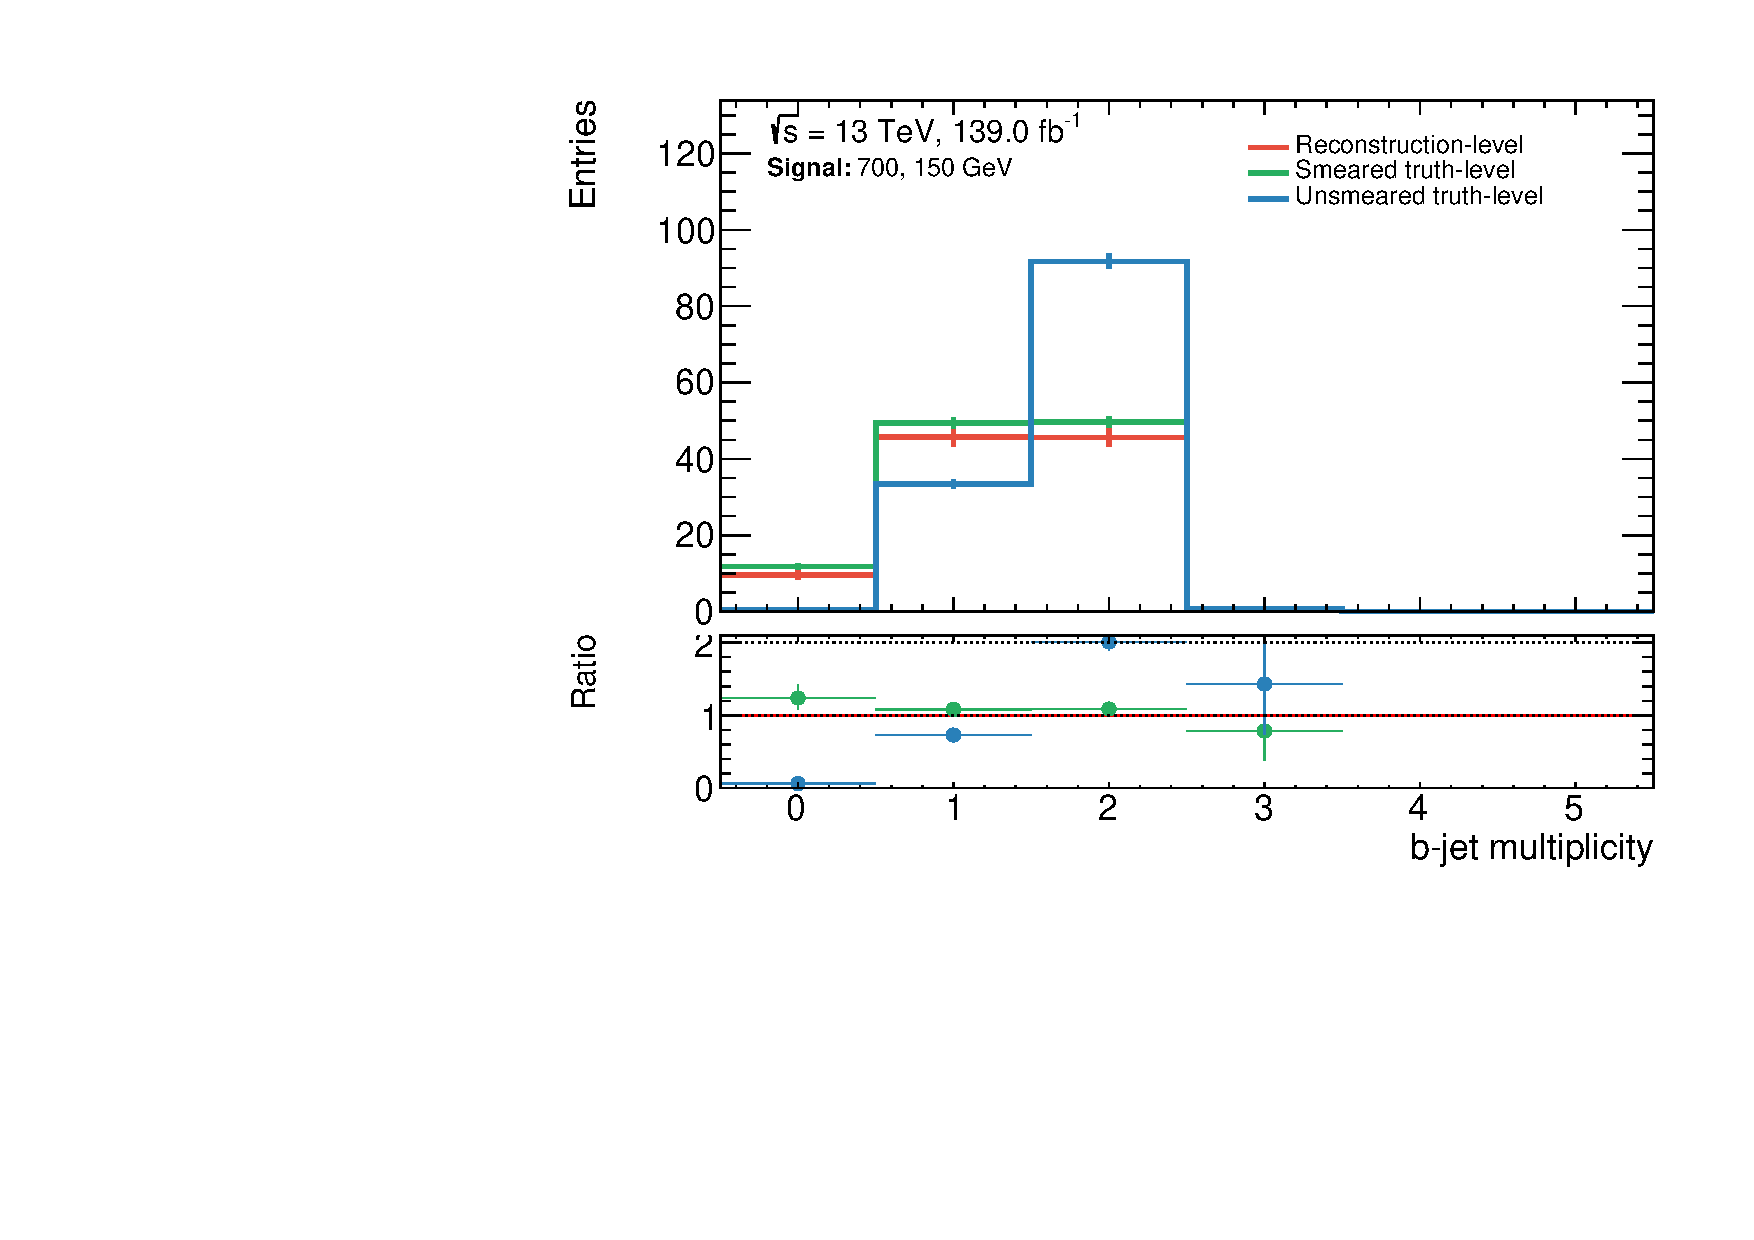
\includegraphics[width=\textwidth]{nBJet30_C1N2_Wh_hbb_700p0_150p0_smeared.pdf}
	\end{subfigure}\hfill
	\caption{Comparisons of the kinematic distributions of key observables at (smeared) truth- and reconstruction-level. The exemplary benchmark signal point with $m(\charg/\neutr), m(\lsp) = 700, \SI{150}{\GeV}$ is shown. The ratio pad shows the ratio between smeared and unsmeared truth-level distributions (green and blue) to reconstruction-level distributions (red). Only \gls{mc} statistical uncertainty is included in the error bars. All distributions are shown in a loose preselection requiring exactly one lepton, $\met>\SI{50}{\GeV}$, $\mt > \SI{50}{\GeV}$, and 2--3 jets, two of which need to be \textit{b}-tagged. The latter requirement is dropped for the \textit{b}-jet multiplicity distribution.}
	\label{fig:smearing_preselection}
\end{figure}
 

 The performance of the truth smearing is illustrated in a loose preselection for a single exemplary benchmark signal point in~\cref{fig:smearing_preselection}. The loose preselection applied requires exactly one lepton, $\met>\SI{50}{\GeV}$, $\mt > \SI{50}{\GeV}$, and 2--3 jets, two of which need to be \textit{b}-tagged. The truth-level distributions are compared with the reconstruction-level distributions before and after truth smearing. It can clearly be observed that the truth smearing noticeably improves the agreement between the truth- and reconstruction-level distributions. While the lepton and jet reconstruction and identification efficiencies are---due to their general dependence on $\eta$, $\pt$ and individual working points---crucial for the overall agreement in shape, the inclusion of flavour-tagging efficiencies significantly improves the overall agreement in normalisation.
 
Although some minor differences remain, overall a good agreement is observed across all relevant kinematic distributions at loose preselection level. Most of the differences between smeared truth-level and reconstruction-level distributions in individual bins are well within the \gls{mc} statistical uncertainties arising from the relatively limited \gls{mc} statistics available.
 
 \subsection{Validation in signal regions}

 \begin{figure}
	\centering
	\begin{subfigure}[b]{0.49\linewidth}
		\centering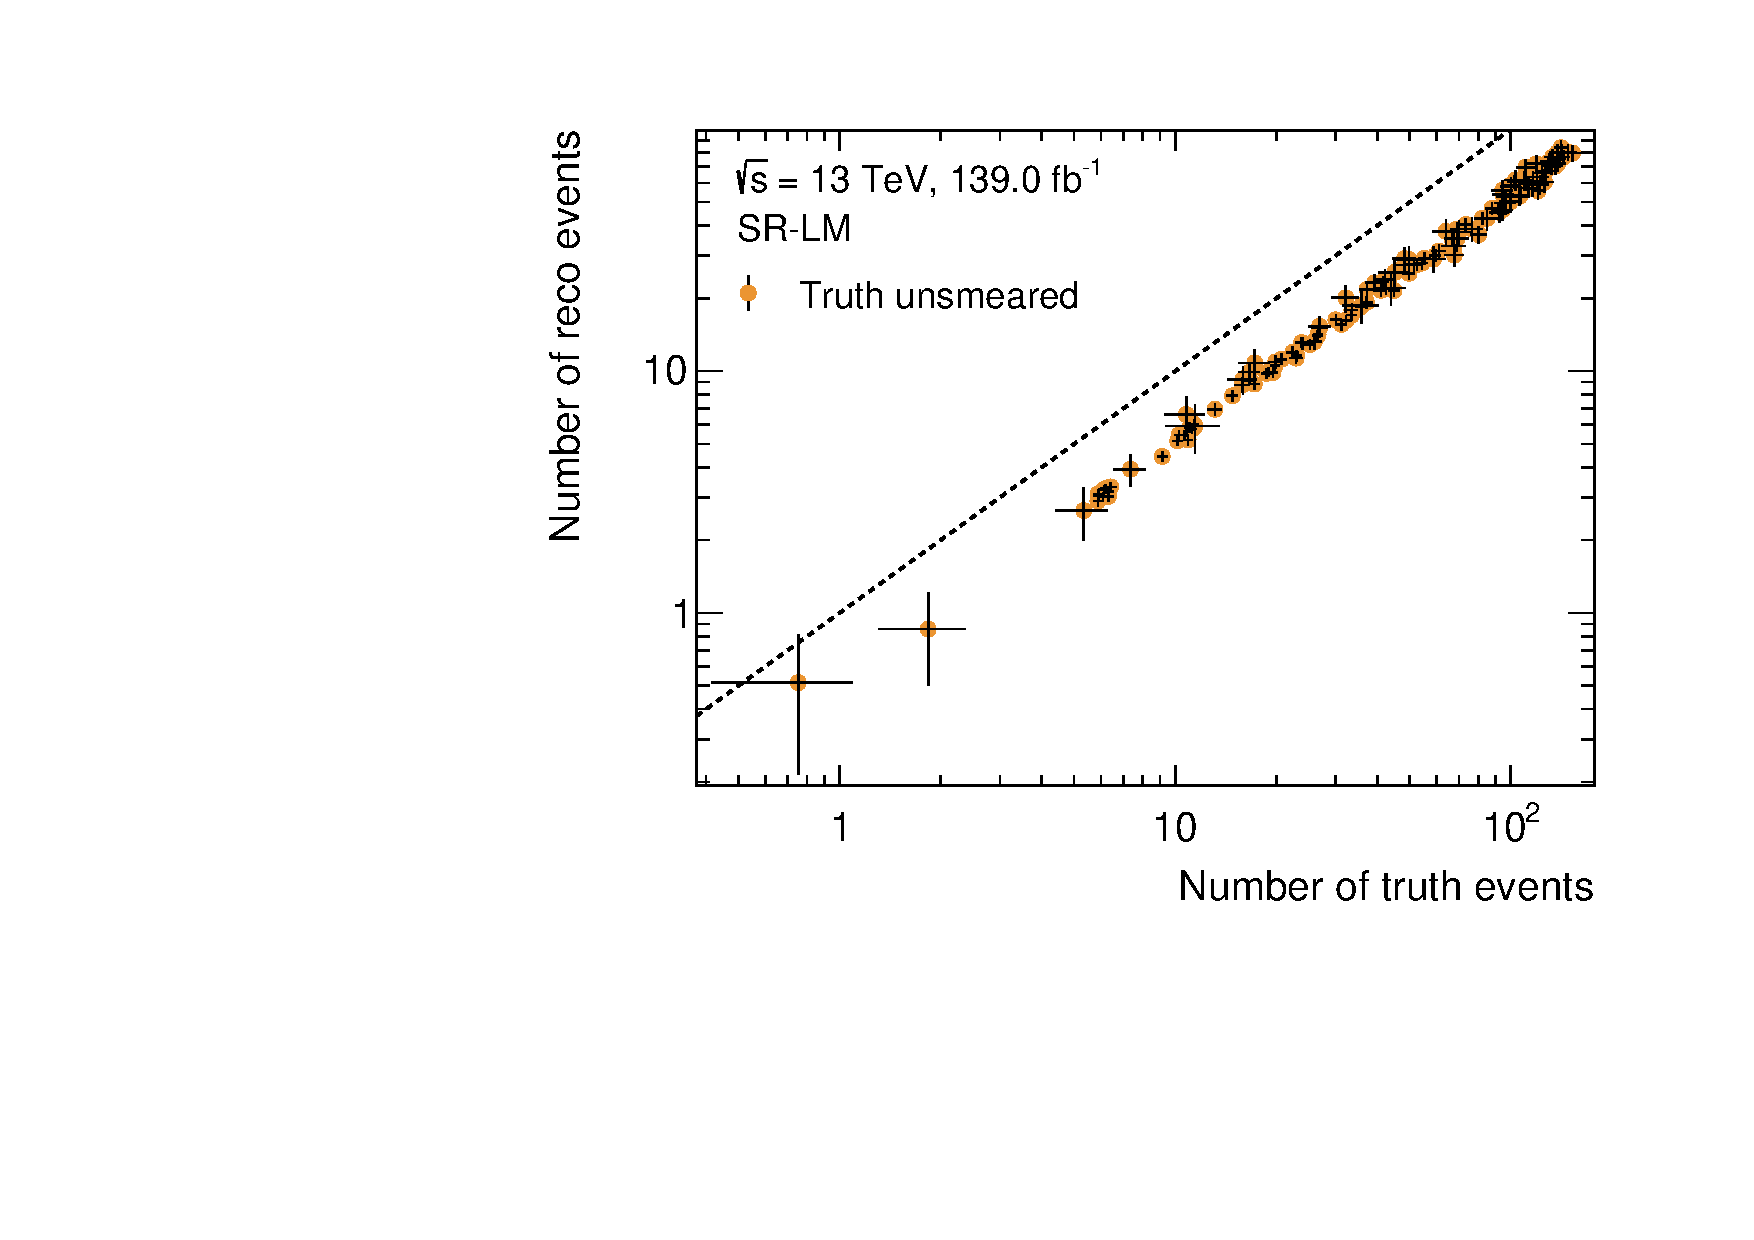
\includegraphics[width=\textwidth]{yields_SR-LM_unsmeared}
	\end{subfigure}\hfill
	\begin{subfigure}[b]{0.49\linewidth}
		\centering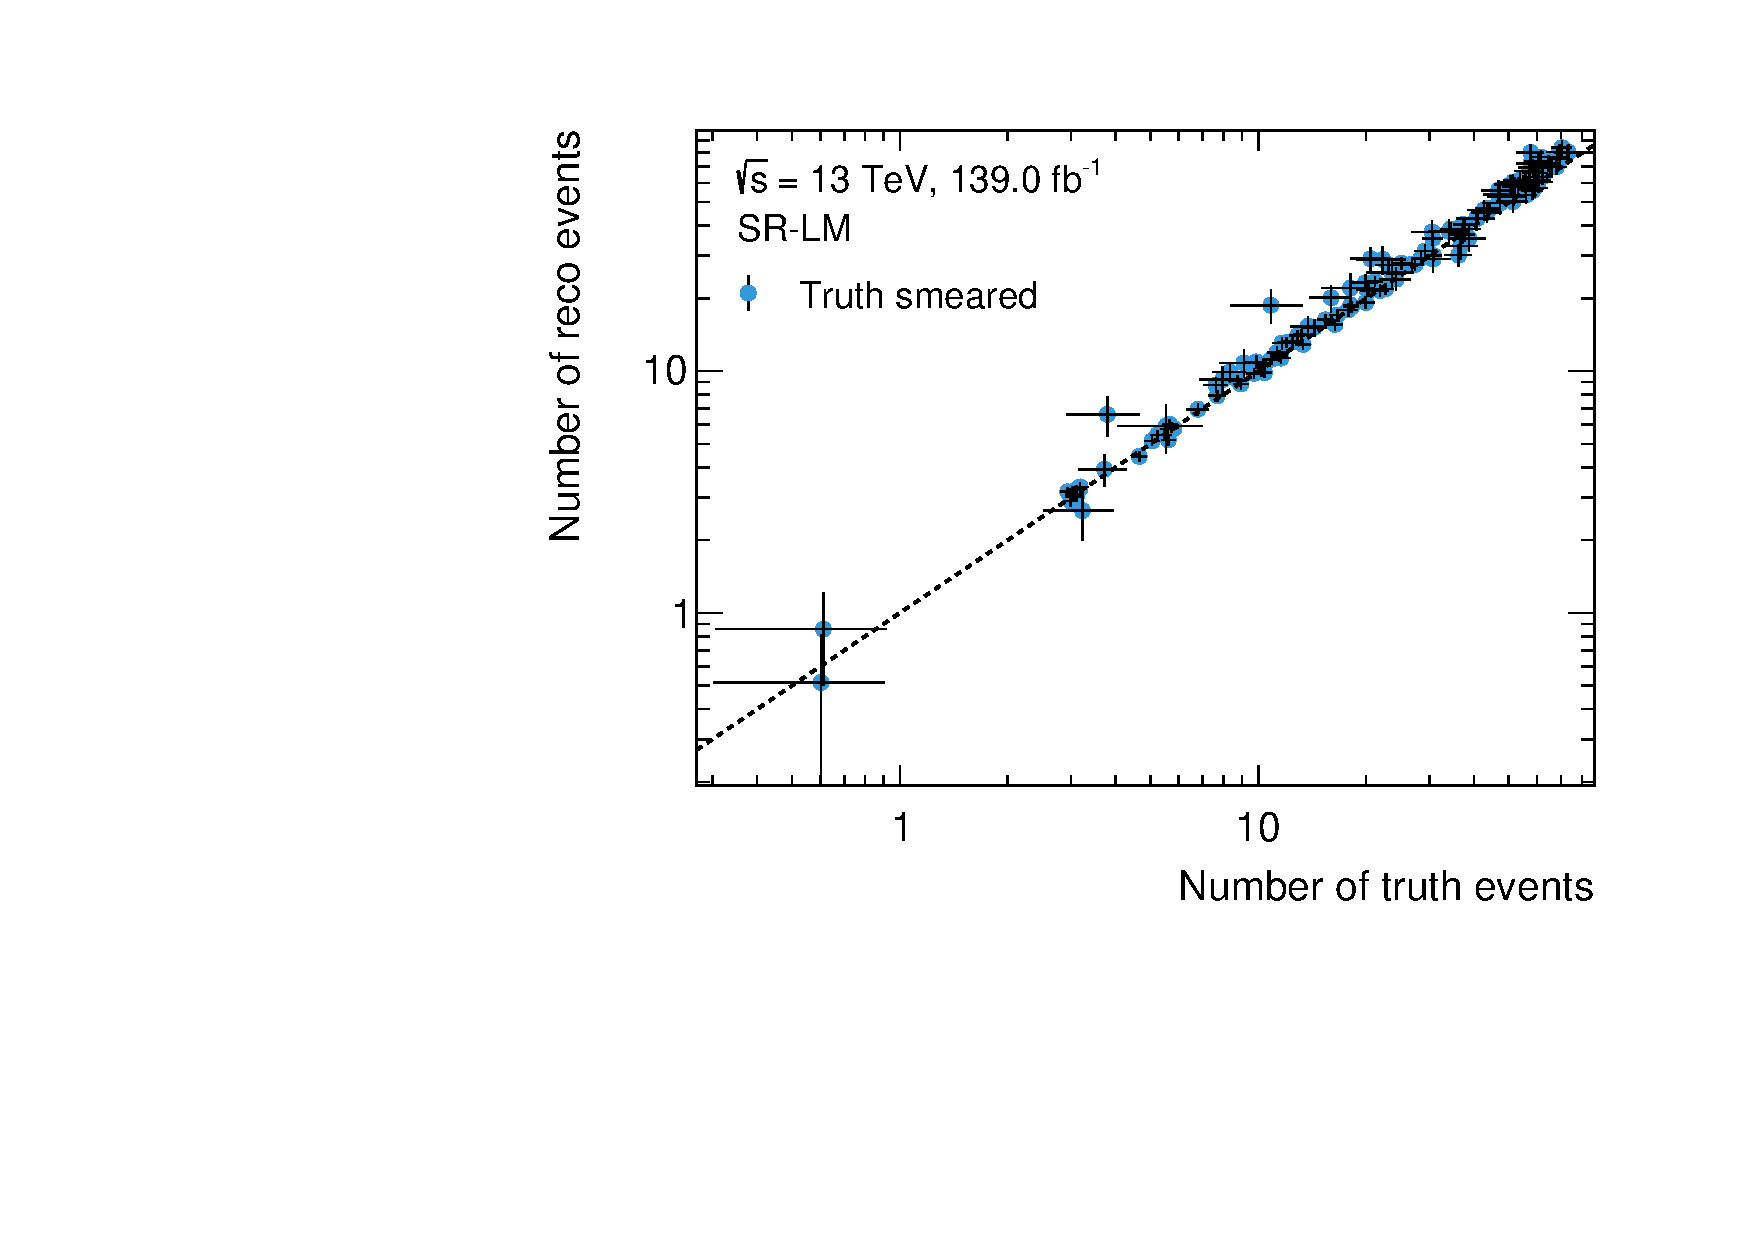
\includegraphics[width=\textwidth]{yields_SR-LM_smeared}
	\end{subfigure}\hfill
	\begin{subfigure}[b]{0.49\linewidth}
		\centering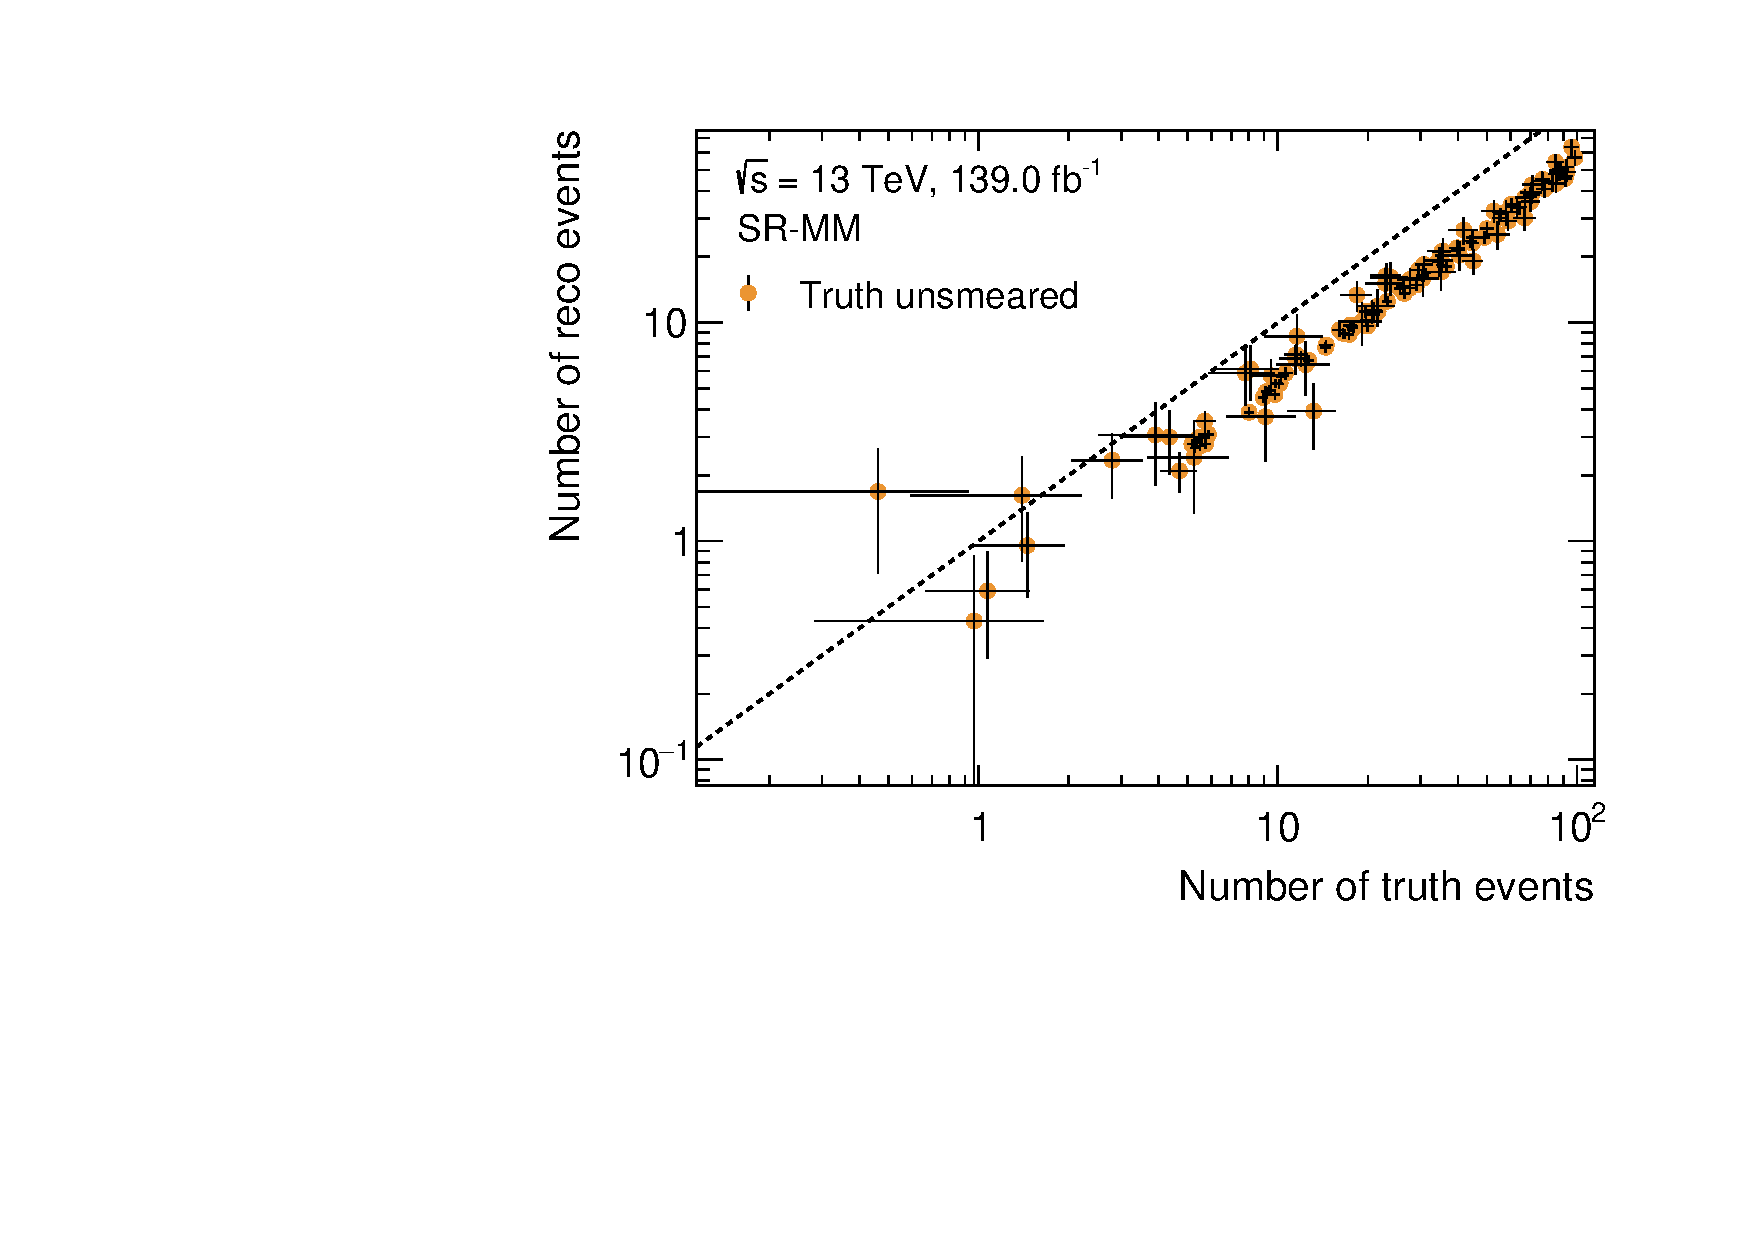
\includegraphics[width=\textwidth]{yields_SR-MM_unsmeared}
	\end{subfigure}\hfill
	\begin{subfigure}[b]{0.49\linewidth}
		\centering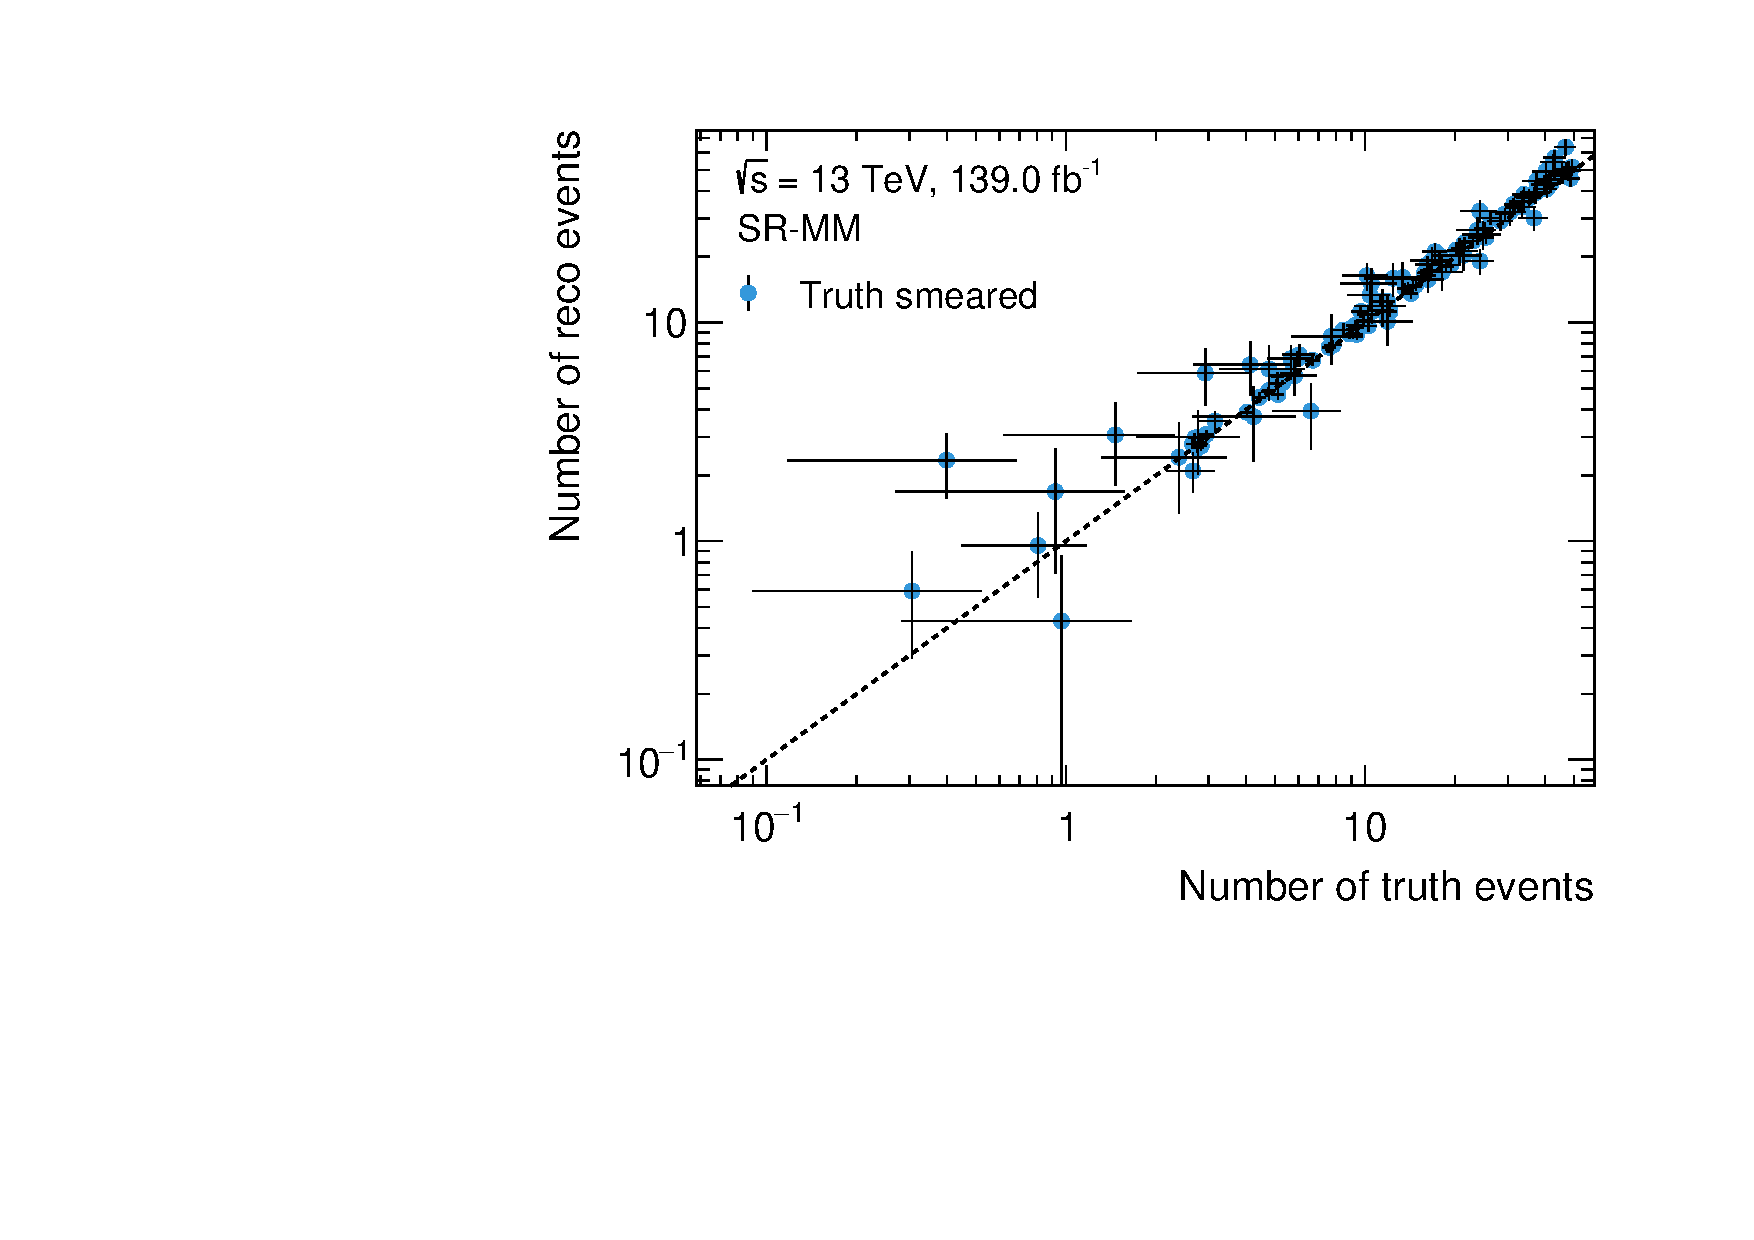
\includegraphics[width=\textwidth]{yields_SR-MM_smeared}
	\end{subfigure}\hfill
	\begin{subfigure}[b]{0.49\linewidth}
		\centering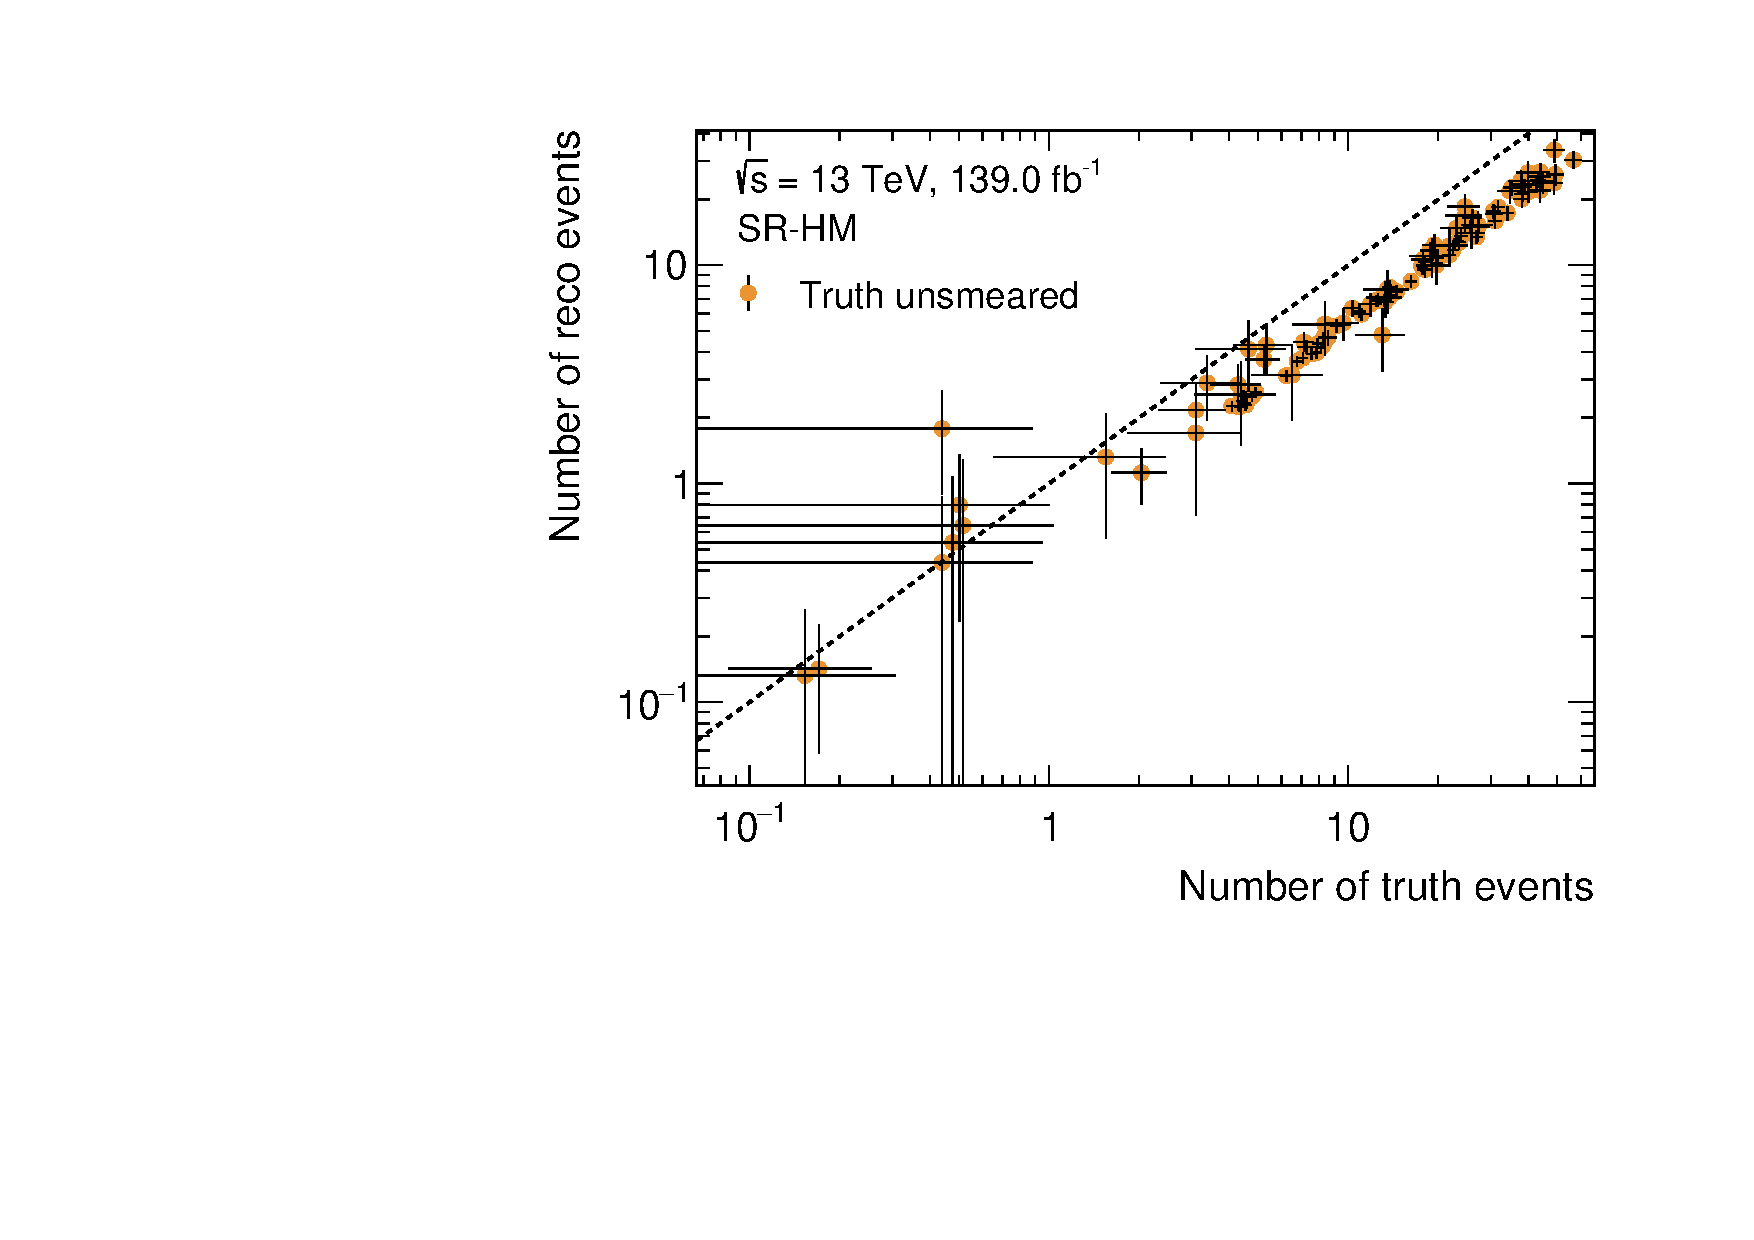
\includegraphics[width=\textwidth]{yields_SR-HM_unsmeared}
	\end{subfigure}\hfill
	\begin{subfigure}[b]{0.49\linewidth}
		\centering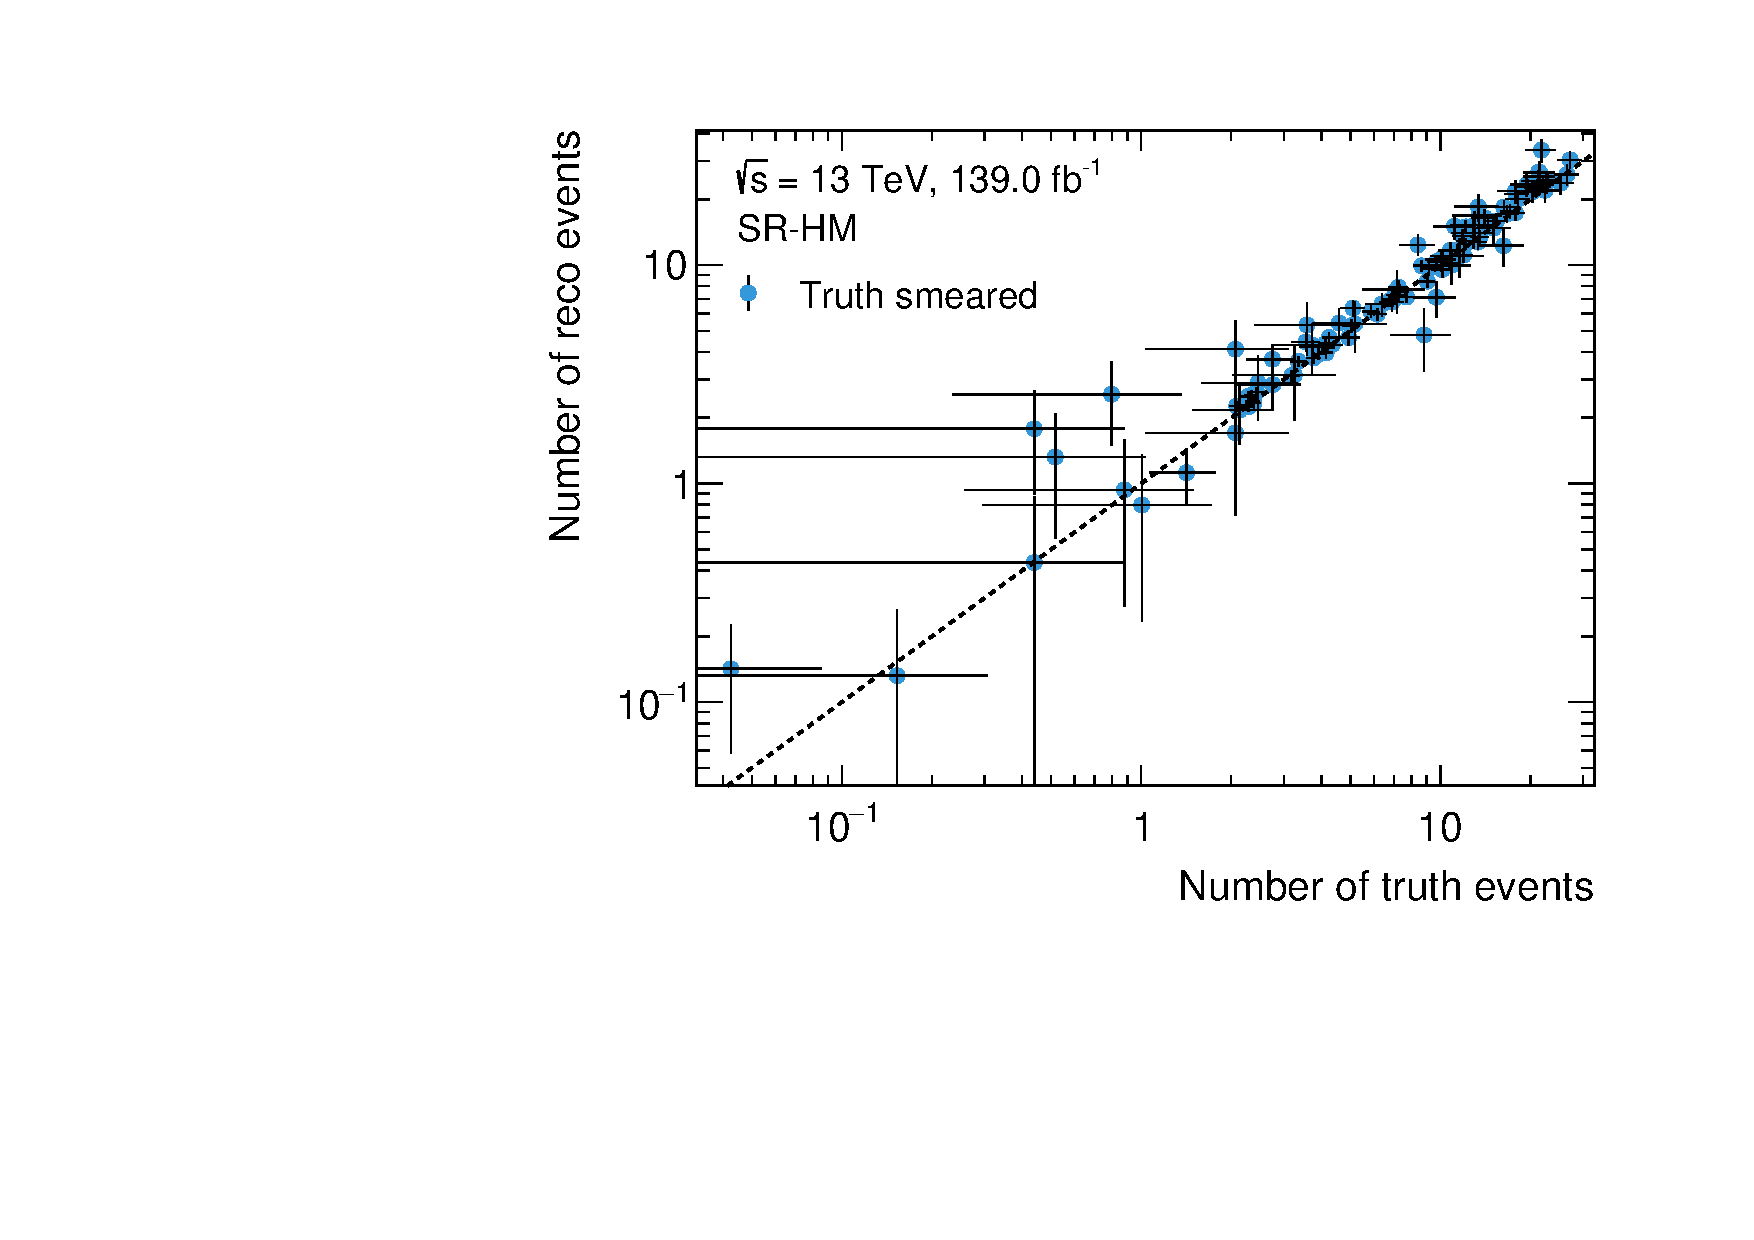
\includegraphics[width=\textwidth]{yields_SR-HM_smeared}
	\end{subfigure}
	\caption{Comparison of the event rates at truth- and reconstruction-level before (left) and after (right) truth smearing. From top to bottom, the SR-LM, SR-MM and SR-HM signal regions are shown, with cumulative (integrated) $\mct$ bins. Every single point in the scatter plots represents a single signal model considered in the original 1-lepton analysis. Uncertainties include \gls{mc} statistical uncertainties.}
	\label{fig:smearing_signal_regions}
\end{figure}
 
 As the expected signal rates in the signal regions are ultimately what is entering the (simplified) likelihood, it is important that the good agreement observed at preselection is still present in the kinematically tight selections of the signal regions. Additionally, it is worth investigating the agreement across all signal models considered in the original analysis. A comparison of the truth-level and reconstruction-level event rates before and after smearing in the signal regions SR-LM, SR-MM and SR-HM is shown in~\cref{fig:smearing_signal_regions} for all signal models considered in the 1-lepton analysis. Only the cumulative $\mct$ bins are shown in each \gls{sr} in~\cref{fig:smearing_signal_regions}. The agreement in the individual $\mct$ bins in each SR-LM, SR-MM and SR-HM is shown in~\cref{fig:smearing_signal_regions_1,fig:smearing_signal_regions_2,fig:smearing_signal_regions_3}.
 
 It can clearly be seen that the truth smearing drastically improves the agreement in event rate estimates at truth- and reconstruction-level across all \gls{sr} bins considered. While the event rates are generally overestimated at truth-level before smearing, compared to reconstruction-level, both tend to agree well within statistical uncertainties after smearing. 
 
\subsection{Validation using simplified likelihood}

Using the expected event rates at smeared truth-level for every signal model in the original signal grid considered in the 1-lepton analysis, expected and observed CL$_s$ values can be computed and exclusion contours can be derived. \Cref{fig:simplified_truth_result} compares the expected and observed exclusion contours obtained using the simplified likelihood and smeared truth-level signal inputs with those obtained using the full likelihood and reconstruction-level signal inputs. Even though---with the simplified likelihood and the smeared truth-level inputs---a significant two-fold approximation is made, the agreement is overall quite good and the published exclusion contour can be reproduced to a relatively high degree of precision. 

In summary, this validation process shows that the signal pipeline in~\cref{fig:pipeline_analysis} can be efficiently approximated using truth-level analysis and a simplified treatment of the statistical model, allowing a considerably faster evaluation of \gls{bsm} models while still offering reliable results. \improvement{CLs plot?}

\begin{figure}
\floatbox[{\capbeside\thisfloatsetup{capbesideposition={right,center},capbesidewidth=0.35\textwidth}}]{figure}[\FBwidth]
{\caption{}\label{fig:simplified_truth_result}}
{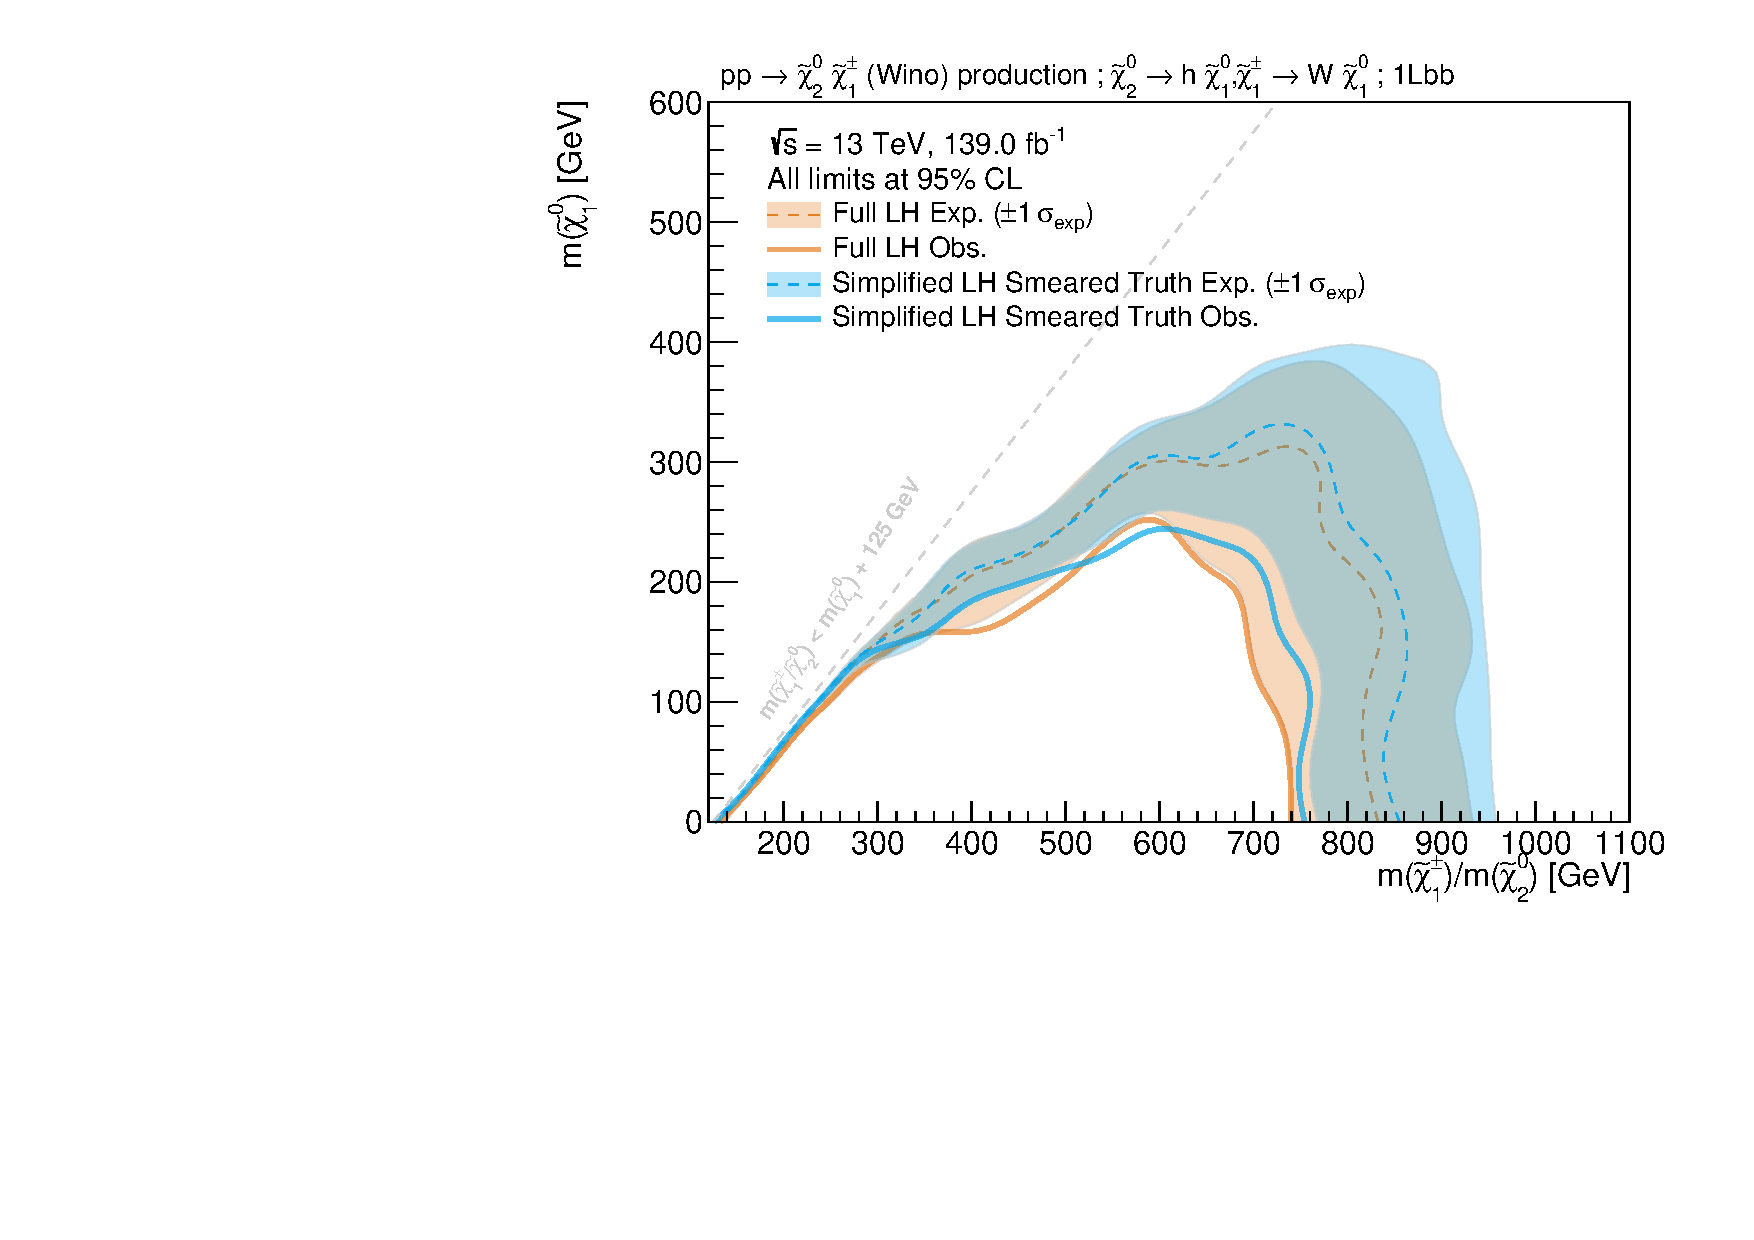
\includegraphics[width=0.60\textwidth]{exclusion_1Lbb_truthInput_BkgSignal_700_200_noLabel}}
\end{figure}

\section{Model sampling and processing}\label{sec:pmssm_sampling}


\subsection{Sampling}

\begin{table}[h]
	\centering
	\small
	\caption{Scan ranges used for each of the 19 pMSSM parameters. For parameters written with a modulus sign, both the positive and negative values are allowed. The term ``gen(s)'' refers to generation(s).}
	\setlength\heavyrulewidth{0.2ex}
	\begin{tabular} {l r r l}
		\toprule
		Parameter & min & max & Note \\ 
		\midrule
		$m_{\tilde{L}_1}$ $(=m_{\tilde{L}_2})$ & $\SI{10}{\TeV}$ & $\SI{10}{\TeV}$ & Left-handed slepton (first two gens.) mass \\
		$m_{\tilde{e}_1}$ $(=m_{\tilde{e}_2})$ & $\SI{10}{\TeV}$ & $\SI{10}{\TeV}$ & Right-handed slepton (first two gens.) mass \\ 
		$m_{\tilde{L}_3}$ & $\SI{10}{\TeV}$ & $\SI{10}{\TeV}$ & Left-handed stau doublet mass \\
		$m_{\tilde{e}_3}$ & $\SI{10}{\TeV}$ & $\SI{10}{\TeV}$ & Right-handed stau mass \\
		\midrule
		$m_{\tilde{Q}_1}$ $(=m_{\tilde{Q}_2})$ & $\SI{10}{\TeV}$ & $\SI{10}{\TeV}$ & Left-handed squark (first two gens.) mass \\
		$m_{\tilde{u}_1}$ $(=m_{\tilde{u}_2})$ & $\SI{10}{\TeV}$ & $\SI{10}{\TeV}$ & Right-handed up-type squark (first two gens.) mass \\
		$m_{\tilde{d}_1}$ $(=m_{\tilde{d}_2})$ &$\SI{10}{\TeV}$ & $\SI{10}{\TeV}$ & Right-handed down-type squark (first two gens.) mass \\
		$m_{\tilde{Q}_3}$ & $\SI{2}{\TeV}$ & $\SI{5}{\TeV}$ & Left-handed squark (third gen.) mass \\
		$m_{\tilde{u}_3}$ & $\SI{2}{\TeV}$ & $\SI{5}{\TeV}$ & Right-handed top squark mass \\
		$m_{\tilde{d}_3}$ & $\SI{2}{\TeV}$ & $\SI{5}{\TeV}$ & Right-handed bottom squark mass \\
		\midrule
		$\vert M_1\vert$ & $\SI{0}{\TeV}$ & $\SI{2}{\TeV}$ & Bino mass parameter \\
		$\vert M_2\vert$ & $\SI{0}{\TeV}$ & $\SI{2}{\TeV}$ & Wino mass parameter \\
		$\vert\mu\vert$ & $\SI{0}{\TeV}$ & $\SI{2}{\TeV}$ & Bilinear Higgs mass parameter \\
		$M_3$ & $\SI{1}{\TeV}$ & $\SI{5}{\TeV}$ & Gluino mass parameter \\
		\midrule
		$\vert A_t\vert$ & $\SI{0}{\TeV}$ & $\SI{8}{\TeV}$ & Trilinear top coupling \\
		$\vert A_b\vert$ & $\SI{0}{\TeV}$ & $\SI{2}{\TeV}$ & Trilinear bottom coupling \\
		$\vert A_\tau\vert$ & $\SI{0}{\TeV}$ & $\SI{2}{\TeV}$ & Trilinear $\tau$ lepton coupling \\
		$M_A$ & $\SI{0}{\TeV}$ & $\SI{5}{\TeV}$ & Pseudoscalar Higgs boson mass \\
		$\tan\beta$ & $1$ & $60$ & Ratio of the Higgs vacuum expectation values \\
		\bottomrule
	\end{tabular}

	\label{fig:pmssm_scan_ranges}   
\end{table}

All signal models considered in the following are sampled from the \gls{pmssm} using the parameter ranges shown in~\cref{fig:pmssm_scan_ranges}. Flat probability distributions are used to draw random values within the given ranges for each parameter and each unique set of \gls{pmssm} parameters generated that way is referred to as an independent \gls{susy} model. 

As this work discusses a search for electroweakinos, the \gls{susy} models drawn from the \gls{pmssm} are sampled with a special focus on said supersymmetric particles. This is achieved by setting the mass parameters of the first and second generation squarks as well as those of the sleptons to values much higher than those accessible at \gls{lhc} energies, effectively decoupling them. For naturalness arguments, third generation squarks and the gluino are not strictly decoupled but set to sufficiently high values such as not to affect the electroweak sector too much. The lower and upper bounds on the 12 scanned parameters are chosen to yield a high density of models with electroweakino masses accessible at \gls{lhc} energies. 

Once a value for each of the 19 \gls{pmssm} parameters has been chosen, a number of publicly available software packages are executed in order to compute the properties of each model point. In a first step, \textsc{SPheno}~v4.0.5~\cite{spheno_1:2003um,spheno_2:2011nf} is used to calculate the spectrum of the sparticles. The result of \textsc{SPheno} is used to determine the masses and mixings of the Higgs bosons using \textsc{FeynHiggs}~v2.16.0~\cite{FeynHiggs:1998yj,FeynHiggs_1:2018qog,FeynHiggs_2:2013ria}, after which \textsc{SPheno} is re-executed in order to update the rest of the sparticle spectrum. An additional \gls{susy} spectrum calculation is performed with \textsc{SoftSusy}~v4.1.10~\cite{softsusy:2001kg}. Although the masses, mixings and branching fractions from \textsc{SoftSusy} will not directly be used in the following, the program is still required to complete successfully in order to reduce the number of \gls{pmssm} models with pathological properties. After the complete model spectrum has calculated, additional properties are determined. The dark matter relic abundance of each model is calculated with \textsc{micrOMEGAs}~v5.2.1~\cite{micromegas_1:2006is,micromegas_2:2010pz}. Finally, flavour physics and precision electroweak observables like $\Delta\rho$, $\Delta(g-2)_\mu$, $\mathrm{BR}(b\rightarrow s\gamma)$ and $\mathrm{BR}(B_s\rightarrow \mu^+\mu^-)$ are determined using \textsc{GM2Calc}~v1.7.1~\cite{gm2:2015rva} and \textsc{SuperIso}~v4.0~\cite{superiso:2008tp}.

\subsection{Selection and processing}

A total of \num[group-separator={,}]{200000} unique models are sampled from the \gls{pmssm} using the above prescription. After requiring all spectrum generators and properties calculations to finish without errors as well as models to produce a dark matter relic density satisfying $\Omega_c h^2 < 0.12$, a total of \num[group-separator={,}]{106854} models survive. The cross section for all surviving models is computed at \gls{nlo} using \textsc{Prospino}~v2.1~\cite{prospino:314229, prospino_2:1999xh}. Models with an inclusive cross sections for all electroweak production processes below $\SI{0.07}{\femto\barn}$ are discarded as they would result in less than 10 expected signal events with an integrated luminosity of \onethirtynineifb, not enough to be sensitive to with current electroweak \gls{susy} searches. Models are also discarded for lack of experimental sensitivity if the $\charg$ is heavier than $\SI{1.2}{\TeV}$. Next, models are only considered in the following if their \gls{lsp} is the $\lsp$. Finally, models with long-lived or even stable (on the time scale needed for traversing the ATLAS detector) sparticles\footnote{Not considering the \gls{lsp}.} are discarded as \gls{susy} searches targeting prompt electroweakino decays (like the 1-lepton search), are not expected to be sensitive to these models. 

Altogether, \num[group-separator={,}]{90974} of the \gls{pmssm} models sampled satisfy all constraints and are generated at truth-level in a subsequent step. 

\subsection{Event generation}

Event generation is performed using the software centrally provided by the ATLAS production system. The initial pair of sparticles with two one parton in the \gls{me} are generated using the \textsc{MadGraph5\_aMC@NLO} v2.6.1.~\cite{MGaMCNLO:2014hca,Frederix:2012ps} generator. Next, \textsc{Pythia8.230}~\cite{Pythia8:2007gs}  with the \textsc{A14} tune is used for the hadronisation and \gls{ps}, together with the NNPDF 2.3 LO~\cite{Ball:2012cx} \gls{PDF} set.
		
\subsection{Truth-level analysis}

All models passing event generation are evaluated using the truth-level analysis described in~\cref{sec:truth_analysis}.


\section{Results in the pMSSM}
